% vim: spell spelllang=en:
%! TEX root = **/main.tex
\documentclass[12pt, oneside]{article}
\usepackage[a4paper, left=2.5cm, right=2.5cm, top=2.5cm, bottom=2.5cm]{geometry}

\usepackage[T1]{fontenc}
\usepackage[utf8]{inputenc} % Use unicode for input
%\usepackage{lmodern}

\usepackage[english]{babel}

%% Bibliography:
%\usepackage{comment}
%\usepackage[
    %backend=biber,
    %style=numeric,
%]{biblatex}
%\DeclareNameAlias{default}{last-first}

%\usepackage{csquotes}       % For bibliography quotations
%\DeclareQuoteAlias{spanish}{catalan}

%\addbibresource{biblio.bib}
%% see:
%% https://www.sharelatex.com/learn/Bibliography_management_in_LaTeX#The_bibliography_file

%\usepackage{datetime} % Customize date
%% \monthyeardate\today gives the date without the day
%\newdateformat{monthyeardate}{%
    %\monthname[\THEMONTH], \THEYEAR}

% For cross references
\usepackage{xcolor}
\usepackage{color}
\usepackage[colorlinks = true]{hyperref}
\usepackage[english]{varioref}
%\usepackage{cleveref}
%hyperref configuration so that it doesn't contrast so much colorlinks,
\hypersetup{
   linkcolor={black},
   citecolor={black},
   %linkcolor={red!50!black},
   %citecolor={blue!50!black},
   urlcolor={blue!80!black}
}

\usepackage{mathtools}  % amsmath + more
\usepackage{amsthm}     % Theorem enviroment
\usepackage{amssymb}    % More symbols
\usepackage{amstext}    % Text inside mathenv

\usepackage{relsize}    % Bigger math with mathlarger{___}
\usepackage{nicefrac}   % nice fractions in one line

\usepackage[export]{adjustbox}  % Adjust table size
\usepackage{float}              % Force tables and images position (H and H!)
\usepackage{wrapfig}            % Wrap images like in HTML

%\usepackage{tabularx, colortbl, booktabs}    % Better tables
%\usepackage{tabularx, colortbl, booktabs}    % Better tables
%\usepackage{longtable}                      % Multiple page table
\usepackage{xltabular}
\usepackage{colortbl, booktabs}    % Better tables

% bug booktabs + xltabular
\makeatletter
\def\@BTrule[#1]{%
  \ifx\longtable\undefined
    \let\@BTswitch\@BTnormal
  \else\ifx\hline\LT@hline
    \nobreak
    \let\@BTswitch\@BLTrule
  \else
     \let\@BTswitch\@BTnormal
  \fi\fi
  \global\@thisrulewidth=#1\relax
  \ifnum\@thisruleclass=\tw@\vskip\@aboverulesep\else
  \ifnum\@lastruleclass=\z@\vskip\@aboverulesep\else
  \ifnum\@lastruleclass=\@ne\vskip\doublerulesep\fi\fi\fi
  \@BTswitch}
\makeatother

% Split cell in lines and more formating options inside table
\usepackage{array, multirow, multicol, makecell}

%\usepackage{subcaption}                     % Subfigures
%\usepackage[framemethod=tikz]{mdframed}     % Custom frames

%\usepackage[bottom]{footmisc} % Footnotes at bottom of page

%\usepackage[alsoload=hep]{siunitx}          % SI units and uncertainties
%\sisetup{locale = FR}                       % Commas and so on for spanish
%\sisetup{separate-uncertainty=true}
%\sisetup{
  %per-mode=fraction,
  %fraction-function=\nicefrac
%}

%\usepackage{tikz}
%%\usetikzlibrary{arrows}
%%\usetikzlibrary{scopes}
%\usetikzlibrary{babel}

%\usepackage{listings}       % For code blocks

%% Custom code highlight
%\definecolor{codegreen}{rgb}{0,0.6,0}
%\definecolor{codegray}{rgb}{0.5,0.5,0.5}
%\definecolor{codepurple}{rgb}{0.58,0,0.82}
%\definecolor{backcolour}{rgb}{0.95,0.95,0.92}
%\definecolor{lightblue}{RGB}{135,206,250}

%\lstdefinestyle{mystyle}{ backgroundcolor=\color{backcolour},
    %commentstyle=\color{codegreen}, keywordstyle=\color{blue},
    %numberstyle=\tiny\color{codegray}, stringstyle=\color{red},
    %identifierstyle=\color{black}, basicstyle=\footnotesize,
    %%breakatwhitespace=false,
    %breaklines=true,
    %%captionpos=b,                    keepspaces=true,
    %numbers=left,                    numbersep=5pt,
    %showspaces=false,
    %%showstringspaces=false, showtabs=false,
    %tabsize=4
%}
%\lstset{style=mystyle}

\newcommand{\whitepage}{
    \clearpage\thispagestyle{empty}\addtocounter{page}{-1} \newpage \clearpage
}

% Add command before appendix session for page numbering: A-1
%\newcommand{\appendixpagenumbering}{
    %\break
    %\pagenumbering{arabic}
    %\renewcommand{\thepage}{\thesection-\arabic{page}}
%}

%% Custom Math operators (functions not in italic in math mode):
%\DeclareMathOperator{\arcsec}{arcsec}
%\DeclareMathOperator{\arccot}{arccot}
%\DeclareMathOperator{\arccsc}{arccsc}
%\DeclareMathOperator{\cis}{cis}

\usepackage{pdflscape}
\usepackage{pifont}

\usepackage{pdfpages}
\usepackage{comment}
\usepackage{xspace}

%! TEX root = **/main.tex
\PassOptionsToPackage{unicode}{hyperref}
\PassOptionsToPackage{hyphens}{url}
%
% \usepackage{lmodern}
% \usepackage{amssymb,amsmath}
\usepackage{ifxetex,ifluatex}
% \ifnum 0\ifxetex 1\fi\ifluatex 1\fi=0 % if pdftex
%   \usepackage[T1]{fontenc}
%   \usepackage[utf8]{inputenc}
%   \usepackage{textcomp} % provide euro and other symbols
% \else % if luatex or xetex
%   \usepackage{unicode-math}
%   \defaultfontfeatures{Scale=MatchLowercase}
%   \defaultfontfeatures[\rmfamily]{Ligatures=TeX,Scale=1}
% \fi
% Use upquote if available, for straight quotes in verbatim environments
\IfFileExists{upquote.sty}{\usepackage{upquote}}{}
\IfFileExists{microtype.sty}{% use microtype if available
  \usepackage[]{microtype}
  \UseMicrotypeSet[protrusion]{basicmath} % disable protrusion for tt fonts
}{}
\makeatletter
% \@ifundefined{KOMAClassName}{% if non-KOMA class
  % \IfFileExists{parskip.sty}{%
    \usepackage{parskip}
  % }{% else
    % \setlength{\parindent}{0pt}
    % \setlength{\parskip}{6pt plus 2pt minus 1pt}}
% }{% if KOMA class
  % \KOMAoptions{parskip=half}}
\makeatother
\usepackage{xcolor}
\IfFileExists{xurl.sty}{\usepackage{xurl}}{} % add URL line breaks if available
\IfFileExists{bookmark.sty}{\usepackage{bookmark}}{\usepackage{hyperref}}
\hypersetup{%
  hidelinks,
  pdfcreator={LaTeX via pandoc}}
\urlstyle{same} % disable monospaced font for URLs
% \usepackage[margin=1in]{geometry}
\usepackage{color}
\usepackage{fancyvrb}
\newcommand{\VerbBar}{|}
\newcommand{\VERB}{\Verb[commandchars=\\\{\}]}
\DefineVerbatimEnvironment{Highlighting}{Verbatim}{commandchars=\\\{\}}
% Add ',fontsize=\small' for more characters per line
\usepackage{framed}
\definecolor{shadecolor}{RGB}{248,248,248}
\newenvironment{Shaded}{\begin{snugshade}}{\end{snugshade}}
\newcommand{\AlertTok}[1]{\textcolor[rgb]{0.94,0.16,0.16}{#1}}
\newcommand{\AnnotationTok}[1]{\textcolor[rgb]{0.56,0.35,0.01}{\textbf{\textit{#1}}}}
\newcommand{\AttributeTok}[1]{\textcolor[rgb]{0.77,0.63,0.00}{#1}}
\newcommand{\BaseNTok}[1]{\textcolor[rgb]{0.00,0.00,0.81}{#1}}
\newcommand{\BuiltInTok}[1]{#1}
\newcommand{\CharTok}[1]{\textcolor[rgb]{0.31,0.60,0.02}{#1}}
\newcommand{\CommentTok}[1]{\textcolor[rgb]{0.56,0.35,0.01}{\textit{#1}}}
\newcommand{\CommentVarTok}[1]{\textcolor[rgb]{0.56,0.35,0.01}{\textbf{\textit{#1}}}}
\newcommand{\ConstantTok}[1]{\textcolor[rgb]{0.00,0.00,0.00}{#1}}
\newcommand{\ControlFlowTok}[1]{\textcolor[rgb]{0.13,0.29,0.53}{\textbf{#1}}}
\newcommand{\DataTypeTok}[1]{\textcolor[rgb]{0.13,0.29,0.53}{#1}}
\newcommand{\DecValTok}[1]{\textcolor[rgb]{0.00,0.00,0.81}{#1}}
\newcommand{\DocumentationTok}[1]{\textcolor[rgb]{0.56,0.35,0.01}{\textbf{\textit{#1}}}}
\newcommand{\ErrorTok}[1]{\textcolor[rgb]{0.64,0.00,0.00}{\textbf{#1}}}
\newcommand{\ExtensionTok}[1]{#1}
\newcommand{\FloatTok}[1]{\textcolor[rgb]{0.00,0.00,0.81}{#1}}
\newcommand{\FunctionTok}[1]{\textcolor[rgb]{0.00,0.00,0.00}{#1}}
\newcommand{\ImportTok}[1]{#1}
\newcommand{\InformationTok}[1]{\textcolor[rgb]{0.56,0.35,0.01}{\textbf{\textit{#1}}}}
\newcommand{\KeywordTok}[1]{\textcolor[rgb]{0.13,0.29,0.53}{\textbf{#1}}}
\newcommand{\NormalTok}[1]{#1}
\newcommand{\OperatorTok}[1]{\textcolor[rgb]{0.81,0.36,0.00}{\textbf{#1}}}
\newcommand{\OtherTok}[1]{\textcolor[rgb]{0.56,0.35,0.01}{#1}}
\newcommand{\PreprocessorTok}[1]{\textcolor[rgb]{0.56,0.35,0.01}{\textit{#1}}}
\newcommand{\RegionMarkerTok}[1]{#1}
\newcommand{\SpecialCharTok}[1]{\textcolor[rgb]{0.00,0.00,0.00}{#1}}
\newcommand{\SpecialStringTok}[1]{\textcolor[rgb]{0.31,0.60,0.02}{#1}}
\newcommand{\StringTok}[1]{\textcolor[rgb]{0.31,0.60,0.02}{#1}}
\newcommand{\VariableTok}[1]{\textcolor[rgb]{0.00,0.00,0.00}{#1}}
\newcommand{\VerbatimStringTok}[1]{\textcolor[rgb]{0.31,0.60,0.02}{#1}}
\newcommand{\WarningTok}[1]{\textcolor[rgb]{0.56,0.35,0.01}{\textbf{\textit{#1}}}}
\usepackage{graphicx}
\makeatletter
\def\maxwidth{\ifdim\Gin@nat@width>\linewidth\linewidth\else\Gin@nat@width\fi}
\def\maxheight{\ifdim\Gin@nat@height>\textheight\textheight\else\Gin@nat@height\fi}
\makeatother
% Scale images if necessary, so that they will not overflow the page
% margins by default, and it is still possible to overwrite the defaults
% using explicit options in \includegraphics[width, height, ...]{}
\setkeys{Gin}{width=\maxwidth,height=\maxheight,keepaspectratio}
% Set default figure placement to htbp
\makeatletter
\def\fps@figure{htbp}
\makeatother
\setlength{\emergencystretch}{3em} % prevent overfull lines
\providecommand{\tightlist}{%
  \setlength{\itemsep}{0pt}\setlength{\parskip}{0pt}}
\setcounter{secnumdepth}{-\maxdimen} % remove section numbering
\ifluatex
  \usepackage{selnolig}  % disable illegal ligatures
\fi


\usepackage{pgfgantt}

\graphicspath{{../..}{..}{../../analysis/anal_files/figure-latex}}

\title{MD - AirBnB Barcelona Listings}
\author{
    Aleix Bon\'e\\
    Eduard Bosch\\
    David Gili\\
    Albert Mercad\'e\\
}
\date{\today}

\begin{document}


% vim: spell spelllang=en:
%! TEX root = **/main.tex
\thispagestyle{empty}
\clearpage
\setcounter{page}{-1}

\begin{titlepage}
{
    \centering
    \null
    \vfill
    {\Large Data Mining\par}
    \vspace{2em}
    {\Huge \bfseries
        Airbnb Barcelona Listings
    \par}
    \vspace{2em}
    {\large \scshape
        UPC
    \par}
    \vfill
\begin{center}

\end{center}
    \vspace{3cm}

    \vfill
    {\raggedleft \large
Aleix Boné\\
Eduard Bosch\\
David Gili\\
Alber Mercadé\\
        \par}
}
\end{titlepage}

\pagebreak

\setcounter{tocdepth}{2}
\tableofcontents

% Initial working plan (two pages): Including Gantt, division of tasks and
% brief risk contingency plan(see Working team resources slides in the website
% section entitled Working team resources)
\clearpage
%\section{Working Plan}
% vim: spell spelllang=en:
%! TEX root = **/main.tex

% Initial working plan (two pages): Including Gantt, division of tasks and
% brief risk contingency plan(see Working team resources slides in the website
% section entitled Working team resources)

\subsection{Gantt}%
\label{sub:gantt}

\subsection{Division of tasks}%
\label{sub:division_of_tasks}

\newcommand*\rot{\rotatebox{90}}
\newcommand*\X{\ding{56}}
\newcommand*\x{\ding{55}}
\begin{table}[H]
\centering
\begin{tabular}{@{}l|c|c|c|c@{}}
             & \rot{Aleix Boné} & \rot{Eduard Bosch} & \rot{David Gili} & \rot{Albert Mercadé} \\
\toprule
\textbf{Coordination}                           &    & \X &    &    \\ \midrule
\textbf{Motivation and Description}             &    &    & \x &    \\ \midrule
\textbf{Data source presentation}               &    &    &    &    \\
Description of data source                      &    &    &    &    \\ \midrule
\textbf{Formal description of data structure}   &    &    &    &    \\
Row descriptions                                &    &    &    &    \\
Metadata Table                                  &    &    &    &    \\
Scope of study                                  &    &    &    &    \\ \midrule
\textbf{Data mining process performed}          &    &    &    &    \\
workflow                                        &    &    &    &    \\ \midrule
\textbf{Description of prepossessing}           &    &    &    &    \\ \midrule
\textbf{Basic statistical descriptive analysis} &    &    &    &    \\
Univariate of all variables                     &    &    &    &    \\
Bivariate when relevant                         &    &    &    &    \\
Descriptives before \& after                    &    &    &    &    \\
Conclusion describing data                      &    &    &    &    \\ \midrule
\textbf{PCA analysis for numerical variables}   &    &    &    &    \\
Scree plot                                      &    &    &    &    \\
Factorial map visualization                     &    &    &    &    \\
\textbf{Hierarchical Clustering}                &    &    &    &    \\ \midrule
Description of data used                        &    &    &    &    \\
Clustering method used                          &    &    &    &    \\
Resulting Dendogram                             &    &    &    &    \\
Discussion about number of clusters            &    &    &    &     \\
Table with description of cluster size          &    &    &    &    \\ \midrule
\textbf{Profiling of clusters}                  &    &    &    &    \\
Profiling graphs                                &    &    &    &    \\
Profiling graphs                                &    &    &    &     \\ \bottomrule
\end{tabular}
\end{table}

\subsection{Risk contingency plan}%
\label{sub:risk_contingency_plan}


\begin{table}[H]
\centering
\begin{tabular}{@{}p{5cm}p{5cm}p{5cm}@{}}
\toprule
Risk & How to prevent & How to manage \\ \midrule
A team member leaves the group & All tasks have at least two members assigned & Pending work reassigned to balance the workload\\
\addlinespace[0.5em]
A team member couldn't complete his assigned tasks one week & All tasks have at least two members assigned & Upon being notified that one member can't fulfill his tasks, the members that share tasks with that person will exceptionally complete his tasks for that week\\
\addlinespace[0.5em]
The project (data \& R scripts) is lost or corrupted & Have multiple back up copies of GitHub repository both on the cloud (Overleaf \& GitLab) and locally in our computers & Recover the whole project from one of the other back ups\\
\bottomrule
\end{tabular}
\end{table}

%
% A fairly complicated example from section 2.9 of the package
% documentation. This reproduces an example from Wikipedia:
% http://en.wikipedia.org/wiki/Gantt_chart
%
\definecolor{barblue}{RGB}{153,204,254}
\definecolor{groupblue}{RGB}{51,102,254}
\definecolor{linkred}{RGB}{165,0,33}
\renewcommand\sfdefault{phv}
\renewcommand\mddefault{mc}
\renewcommand\bfdefault{bc}
\setganttlinklabel{s-s}{START-TO-START}
\setganttlinklabel{f-s}{FINISH-TO-START}
\setganttlinklabel{f-f}{FINISH-TO-FINISH}
\sffamily
\begin{ganttchart}[
    canvas/.append style={fill=none, draw=black!5, line width=.75pt},
    hgrid style/.style={draw=black!5, line width=.75pt},
    vgrid={*1{draw=black!5, line width=.75pt}},
    today=7,
    today rule/.style={
        draw=black!64,
        dash pattern=on 3.5pt off 4.5pt,
        line width=1.5pt
    },
    today label font=\small\bfseries,
    title/.style={draw=none, fill=none},
    title label font=\bfseries\footnotesize,
    title label node/.append style={below=7pt},
    include title in canvas=false,
    bar label font=\mdseries\small\color{black!70},
    bar label node/.append style={left=2cm},
    bar/.append style={draw=none, fill=black!63},
    bar incomplete/.append style={fill=barblue},
    bar progress label font=\mdseries\footnotesize\color{black!70},
    group incomplete/.append style={fill=groupblue},
    group left shift=0,
    group right shift=0,
    group height=.5,
    group peaks tip position=0,
    group label node/.append style={left=.6cm},
    group progress label font=\bfseries\small,
    link/.style={-latex, line width=1.5pt, linkred},
    link label font=\scriptsize\bfseries,
    link label node/.append style={below left=-2pt and 0pt}
    ]{1}{13}
    \gantttitle[
    title label node/.append style={below left=7pt and -3pt}
    ]{WEEKS:\quad1}{1}
    \gantttitlelist{2,...,13}{1} \\
    \ganttgroup[progress=57]{WBS 1 Summary Element 1}{1}{10} \\
    \ganttbar[
    progress=75,
    name=WBS1A
    ]{\textbf{WBS 1.1} Activity A}{1}{8} \\
    \ganttbar[
    progress=67,
    name=WBS1B
    ]{\textbf{WBS 1.2} Activity B}{1}{3} \\
    \ganttbar[
    progress=50,
    name=WBS1C
    ]{\textbf{WBS 1.3} Activity C}{4}{10} \\
    \ganttbar[
    progress=0,
    name=WBS1D
    ]{\textbf{WBS 1.4} Activity D}{4}{10} \\[grid]
    \ganttgroup[progress=0]{WBS 2 Summary Element 2}{4}{10} \\
    \ganttbar[progress=0]{\textbf{WBS 2.1} Activity E}{4}{5} \\
    \ganttbar[progress=0]{\textbf{WBS 2.2} Activity F}{6}{8} \\
    \ganttbar[progress=0]{\textbf{WBS 2.3} Activity G}{9}{10}
    \ganttlink[link type=s-s]{WBS1A}{WBS1B}
    \ganttlink[link type=f-s]{WBS1B}{WBS1C}
    \ganttlink[
    link type=f-f,
    link label node/.append style=left
    ]{WBS1C}{WBS1D}
\end{ganttchart}

%
% A simpler example from the package documentation:
%
\begin{ganttchart}{1}{12}
    \gantttitle{2011}{12} \\
    \gantttitlelist{1,...,12}{1} \\
    \ganttgroup{Group 1}{1}{7} \\
    \ganttbar{Task 1}{1}{2} \\
    \ganttlinkedbar{Task 2}{3}{7} \ganttnewline
    \ganttmilestone{Milestone}{7} \ganttnewline
    \ganttbar{Final Task}{8}{12}
    \ganttlink{elem2}{elem3}
    \ganttlink{elem3}{elem4}
\end{ganttchart}


% Metadata file describing the selection of variables considered for the
% analysis (see slide nr 8 in Data and Metadata slides from Theme 2. Data
% Preparation)
\clearpage
%\begin{landscape}
%\section{Metadata file}
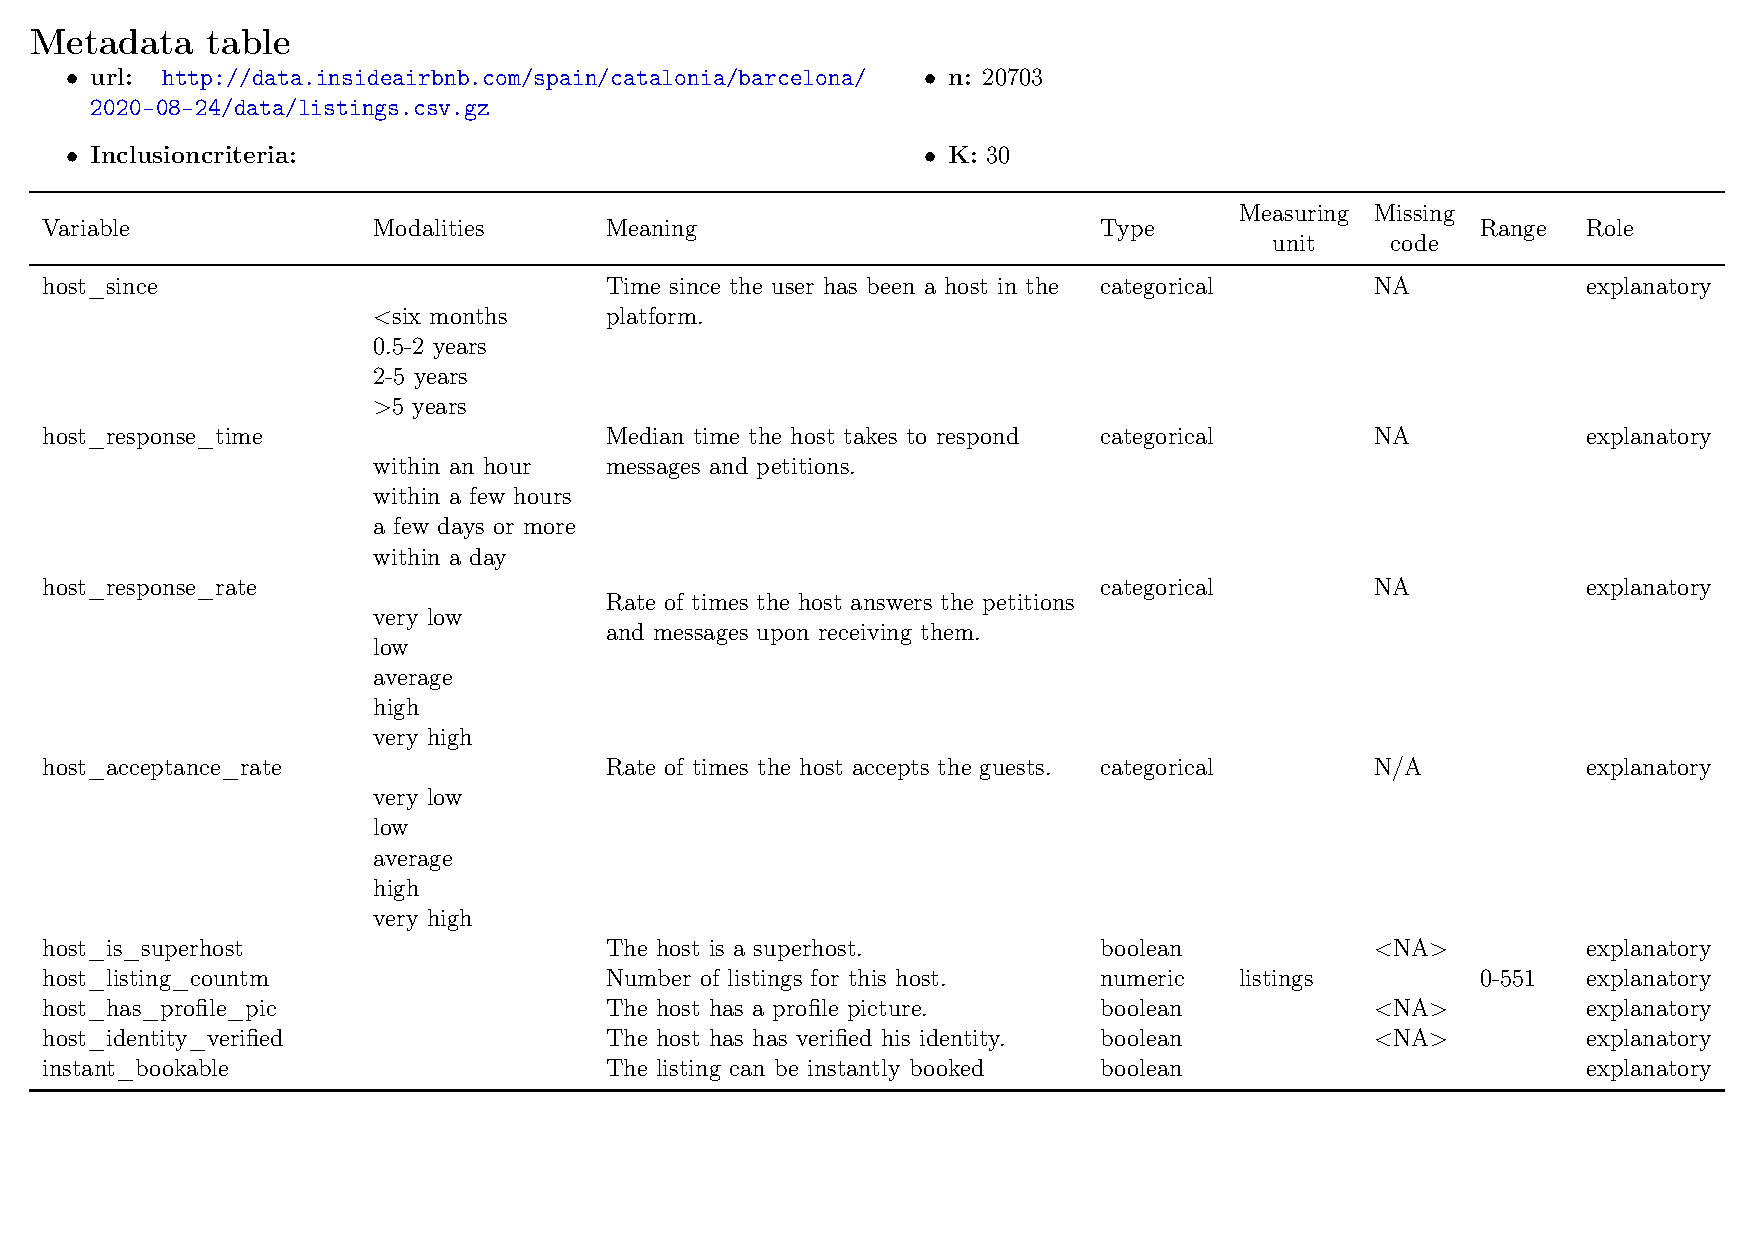
\includepdf[pages=-,landscape=true]{metadata}
%% vim: spell spelllang=en:
%! TEX root = **/main.tex

% Metadata file describing the selection of variables considered for the
% analysis (see slide nr 8 in Data and Metadata slides from Theme 2. Data
% Preparation)

\begin{itemize}
         \item \textbf{url:}
         \item \textbf{Inclusioncriteria:}
         \item \textbf{n:}
         \item \textbf{K:}
\end{itemize}

\begin{center}
\begin{longtable}{@{}lllllllll@{}}
\toprule
Variable & Modalities & meaning & Type & \makecell{Measuring\\ unit} & \makecell{Missing\\ code} & \makecell & Range & Role \\ \midrule
%Variable                    & Modalities                  & meaning                           & Type        & Measuring unit & Missing code                & Measuring procedure & Range   & role \\ \midrule
\endfirsthead
\toprule
Variable & Modalities & meaning & Type & \makecell{Measuring\\ unit} & \makecell{Missing\\ code} & \makecell & Range & Role \\ \midrule

\endhead
\bottomrule
\endfoot
\bottomrule
\endlastfoot

host\_since &                             & \multirow{5}{15ex}{Time since the user has been a host in the platform.} & categorical &                & NA                          &         & role \\
                            & \textless{}six months          &                                   &             &                &                             &                     &         & role \\
                            & 0.5-2 years                  &                                   &             &                &                             &                     &         & role \\
                            & 2-5 years                    &                                   &             &                &                             &                     &         & role \\
                            & \textgreater{}5 years        &                                   &             &                &                             &                     &         & role \\
host\_response\_time        &                             & \multirow{5}{15ex}{Median time the host takes to respond messages and petitions.} & categorical &                & NA                          &                     &         & role \\
                            & within an hour              &                                   &             &                &                             &                     &         & role \\
                            & within a few hours          &                                   &             &                &                             &                     &         & role \\
                            & a few days or more          &                                   &             &                &                             &                     &         & role \\
                            & within a day                &                                   &             &                &                             &                     &         & role \\
host\_response\_rate        &                             & \multirow{5}{15ex}{Rate of times the host answers the petitions and messages upon receiving them.} & categorical &                & NA                    &                     &         & role \\
                            & v.low                       &                                   &             &                &                             &                     &         & role \\
                            & low                         &                                   &             &                &                             &                     &         & role \\
                            & average                     &                                   &             &                &                             &                     &         & role \\
                            & high                        &                                   &             &                &                             &                     &         & role \\
                            & very high                   &                                   &             &                &                             &                     &         & role \\
host\_acceptance\_rate      &                             & \multirow{5}{15ex}{Rate of times the host accepts the guests.} & categorical &                & N/A                         &                     &         & role \\
                            & v.low                       &                                   &             &                &                             &                     &         & role \\
                            & low                         &                                   &             &                &                             &                     &         & role \\
                            & average                     &                                   &             &                &                             &                     &         & role \\
                            & high                        &                                   &             &                &                             &                     &         & role \\
                            & very high                   &                                   &             &                &                             &                     &         & role \\
                            &                             &                                   &             &                &                             &                     &         & role \\
host\_is\_superhost         &                             & The host is a superhost & boolean &                & \textless{}NA\textgreater{} &                     &         & role \\
host\_listing\_count        &                             & Number of listings for this host & numeric     & listings       &                             &                     & 0-551   & role \\
host\_has\_profile\_pic     &                             & t, f & boolean     &                & \textless{}NA\textgreater{} &                     &         & role \\
host\_identity\_verified    &                             & t, f & boolean     &                & \textless{}NA\textgreater{} &                     &         & role \\
neigbourhood\_cleansed      &                             &                                   & categorical &                &                             &                     &         & role \\
                            & Ciutat Vella                &                                   &             &                &                             &                     &         & role \\
                            & Sant Martí                  &                                   &             &                &                             &                     &         & role \\
                            & Gràcia                      &                                   &             &                &                             &                     &         & role \\
                            & Eixample                    &                                   &             &                &                             &                     &         & role \\
                            & Sants-Montjuíc              &                                   &             &                &                             &                     &         & role \\
                            & Sarrià-Sant Gervasi         &                                   &             &                &                             &                     &         & role \\
                            & Les Corts                   &                                   &             &                &                             &                     &         & role \\
                            & Horta-Guinardó              &                                   &             &                &                             &                     &         & role \\
                            & Sant Andreu                 &                                   &             &                &                             &                     &         & role \\
                            & Nou Barris                  &                                   &             &                &                             &                     &         & role \\
room\_type                  &                             &                                   & categorical &                &                             &                     &         & role \\
                            & Private room                &                                   &             &                &                             &                     &         & role \\
                            & Entire home/apt  &                                   &             &                &                             &                     &         & role \\
                                                        & Hotel room  &                                   &             &                &                             &                     &         & role \\

                            & Shared room                 &                                   &             &                &                             &                     &         & role \\
accomodates                 &                             & meaning                           & numerical   & people         &                             &                     & 1-16    & role \\
bedroom                     &                             & meaning                           & numerical   & bedrooms       & NA                          &                     & 1-16    & role \\
bed                         &                             & meaning                           & numerical   & beds           & NA                          &                     & 1-48    & role \\
price                       &                             & meaning                           & numerical   & dollars        &                             &                     & 0-10000 & role \\
minimum\_nights\_averge\_nt &                             & meaning                           & numerical   & nights         &                             &                     & 1-1123  & role \\
maximum\_nights\_averge\_nt &                             & meaning                           & numerical   & nights         &                             &                     & 1-9958  & role \\
availability\_30            &                             & meaning                           & numerical   & days           &                             &                     & 0-30    & role \\
availability\_60            &                             & meaning                           & numerical   & days           &                             &                     & 0-60    & role \\
availability\_90            &                             & meaning                           & numerical   & days           &                             &                     & 0-90    & role \\
availability\_365           &                             & meaning                           & numerical   & days           &                             &                     & 0-365   & role \\
number\_of\_reviews         &                             & meaning                           & numerical   & reviews        &                             &                     & 0-743   & role \\
number\_of\_reviews\_l30d   &                             & meaning                           & numerical   & reviews        &                             &                     & 0-15    & role \\
number\_of\_reviews\_lt     &                             & meaning                           & numerical   & reviews        &                             &                     & 0-278   & role \\
review\_scores\_ratin       &                             & meaning                           & numerical   & stars          &                             &                     & 20-100  & role \\
review\_scores\_accurac     &                             & meaning                           & numerical   & stars          &                             &                     & 2-10    & role \\
review\_scores\_cleanlines  &                             & meaning                           & numerical   & stars          &                             &                     & 2-10    & role \\
review\_scores\_locatio     &                             & meaning                           & numerical   & stars          &                             &                     & 2-10    & role \\
review\_scores\_valu        &                             & meaning                           & numerical   & stars          &                             &                     & 2-10    & role \\
instant\_bookable           &                             & meaning                           & boolean     &                &                             &                     &         & role \\
reviews\_per\_month         &                             & meaning                           & numerical   & reviews        &                             &                     & 0-21.41 & role \\ \bottomrule
\end{longtable}

\end{center}
%\end{landscape}

% Basic initial univariate descriptive statistics of raw variables (see
% provided R scripts for automatic descriptive analysis in  Lab Session2.
% Preprocessing (II). Markdow produces word files, the R script is interpreted.
% The scripts ARE ORIENTATIVE. Modify whenever required)
\clearpage
\section{Descriptive Statistics of raw variables}%
\label{sec:descriptive_analisis}
% vim: spell spelllang=en:
%! TEX root = **/main.tex

% Basic initial univariate descriptive statistics of raw variables (see
% provided R scripts for automatic descriptive analysis in  Lab Session2.
% Preprocessing (II). Markdow produces word files, the R script is interpreted.
% The scripts ARE ORIENTATIVE. Modify whenever required)
{ \centering
Here you can write the introduction of your report and include some text
that will be transferred to the word file every time you re-run this
Markdown

\begin{Shaded}
\begin{Highlighting}[]
\KeywordTok{library}\NormalTok{(viridis)}
\end{Highlighting}
\end{Shaded}

\begin{verbatim}
## Loading required package: viridisLite
\end{verbatim}

\begin{Shaded}
\begin{Highlighting}[]
\KeywordTok{library}\NormalTok{(ggplot2)}

\NormalTok{dd \textless{}{-}}\StringTok{ }\KeywordTok{read.csv}\NormalTok{(}\KeywordTok{gzfile}\NormalTok{(}\StringTok{"../listings.csv.gz"}\NormalTok{), }\DataTypeTok{na.strings =} \KeywordTok{c}\NormalTok{(}\StringTok{""}\NormalTok{, }\StringTok{"N/A"}\NormalTok{))}

\NormalTok{dataset \textless{}{-}}\StringTok{ "airbnb"}
\end{Highlighting}
\end{Shaded}

Check the type of the R object created for the dataset

\begin{Shaded}
\begin{Highlighting}[]
\KeywordTok{class}\NormalTok{(dd)}
\end{Highlighting}
\end{Shaded}

\begin{verbatim}
## [1] "data.frame"
\end{verbatim}

without including the R instruction in the final document

\begin{verbatim}
## [1] "data.frame"
\end{verbatim}

Get dimensions of the dataset

\begin{Shaded}
\begin{Highlighting}[]
\KeywordTok{dim}\NormalTok{(dd)}
\end{Highlighting}
\end{Shaded}

\begin{verbatim}
## [1] 20703    74
\end{verbatim}

\begin{Shaded}
\begin{Highlighting}[]
\NormalTok{n\textless{}{-}}\KeywordTok{dim}\NormalTok{(dd)[}\DecValTok{1}\NormalTok{]}
\NormalTok{K\textless{}{-}}\KeywordTok{dim}\NormalTok{(dd)[}\DecValTok{2}\NormalTok{]}

\NormalTok{n}
\end{Highlighting}
\end{Shaded}

\begin{verbatim}
## [1] 20703
\end{verbatim}

\begin{Shaded}
\begin{Highlighting}[]
\NormalTok{K}
\end{Highlighting}
\end{Shaded}

\begin{verbatim}
## [1] 74
\end{verbatim}

Check the variables

\begin{Shaded}
\begin{Highlighting}[]
\KeywordTok{names}\NormalTok{(dd)}
\end{Highlighting}
\end{Shaded}

\begin{verbatim}
##  [1] "id"                                          
##  [2] "listing_url"                                 
##  [3] "scrape_id"                                   
##  [4] "last_scraped"                                
##  [5] "name"                                        
##  [6] "description"                                 
##  [7] "neighborhood_overview"                       
##  [8] "picture_url"                                 
##  [9] "host_id"                                     
## [10] "host_url"                                    
## [11] "host_name"                                   
## [12] "host_since"                                  
## [13] "host_location"                               
## [14] "host_about"                                  
## [15] "host_response_time"                          
## [16] "host_response_rate"                          
## [17] "host_acceptance_rate"                        
## [18] "host_is_superhost"                           
## [19] "host_thumbnail_url"                          
## [20] "host_picture_url"                            
## [21] "host_neighbourhood"                          
## [22] "host_listings_count"                         
## [23] "host_total_listings_count"                   
## [24] "host_verifications"                          
## [25] "host_has_profile_pic"                        
## [26] "host_identity_verified"                      
## [27] "neighbourhood"                               
## [28] "neighbourhood_cleansed"                      
## [29] "neighbourhood_group_cleansed"                
## [30] "latitude"                                    
## [31] "longitude"                                   
## [32] "property_type"                               
## [33] "room_type"                                   
## [34] "accommodates"                                
## [35] "bathrooms"                                   
## [36] "bathrooms_text"                              
## [37] "bedrooms"                                    
## [38] "beds"                                        
## [39] "amenities"                                   
## [40] "price"                                       
## [41] "minimum_nights"                              
## [42] "maximum_nights"                              
## [43] "minimum_minimum_nights"                      
## [44] "maximum_minimum_nights"                      
## [45] "minimum_maximum_nights"                      
## [46] "maximum_maximum_nights"                      
## [47] "minimum_nights_avg_ntm"                      
## [48] "maximum_nights_avg_ntm"                      
## [49] "calendar_updated"                            
## [50] "has_availability"                            
## [51] "availability_30"                             
## [52] "availability_60"                             
## [53] "availability_90"                             
## [54] "availability_365"                            
## [55] "calendar_last_scraped"                       
## [56] "number_of_reviews"                           
## [57] "number_of_reviews_ltm"                       
## [58] "number_of_reviews_l30d"                      
## [59] "first_review"                                
## [60] "last_review"                                 
## [61] "review_scores_rating"                        
## [62] "review_scores_accuracy"                      
## [63] "review_scores_cleanliness"                   
## [64] "review_scores_checkin"                       
## [65] "review_scores_communication"                 
## [66] "review_scores_location"                      
## [67] "review_scores_value"                         
## [68] "license"                                     
## [69] "instant_bookable"                            
## [70] "calculated_host_listings_count"              
## [71] "calculated_host_listings_count_entire_homes" 
## [72] "calculated_host_listings_count_private_rooms"
## [73] "calculated_host_listings_count_shared_rooms" 
## [74] "reviews_per_month"
\end{verbatim}

Decide if you need to declare some more factor or date

\begin{Shaded}
\begin{Highlighting}[]
\NormalTok{actives\textless{}{-}}\KeywordTok{c}\NormalTok{(}\DecValTok{12}\NormalTok{, }\DecValTok{15}\NormalTok{, }\DecValTok{16}\NormalTok{, }\DecValTok{17}\NormalTok{, }\DecValTok{18}\NormalTok{, }\DecValTok{22}\NormalTok{, }\DecValTok{25}\NormalTok{, }\DecValTok{26}\NormalTok{, }\DecValTok{29}\NormalTok{, }\DecValTok{33}\NormalTok{, }\DecValTok{34}\NormalTok{, }\DecValTok{37}\NormalTok{, }\DecValTok{38}\NormalTok{, }\DecValTok{40}\NormalTok{, }\DecValTok{47}\NormalTok{, }\DecValTok{48}\NormalTok{, }\DecValTok{51}\NormalTok{,}
           \DecValTok{52}\NormalTok{, }\DecValTok{53}\NormalTok{, }\DecValTok{54}\NormalTok{, }\DecValTok{56}\NormalTok{, }\DecValTok{57}\NormalTok{, }\DecValTok{58}\NormalTok{, }\DecValTok{61}\NormalTok{, }\DecValTok{62}\NormalTok{, }\DecValTok{63}\NormalTok{, }\DecValTok{66}\NormalTok{, }\DecValTok{67}\NormalTok{, }\DecValTok{69}\NormalTok{, }\DecValTok{74}\NormalTok{)}

\CommentTok{\# Check variable names}
\KeywordTok{names}\NormalTok{(dd[,actives])}
\end{Highlighting}
\end{Shaded}

\begin{verbatim}
##  [1] "host_since"                   "host_response_time"          
##  [3] "host_response_rate"           "host_acceptance_rate"        
##  [5] "host_is_superhost"            "host_listings_count"         
##  [7] "host_has_profile_pic"         "host_identity_verified"      
##  [9] "neighbourhood_group_cleansed" "room_type"                   
## [11] "accommodates"                 "bedrooms"                    
## [13] "beds"                         "price"                       
## [15] "minimum_nights_avg_ntm"       "maximum_nights_avg_ntm"      
## [17] "availability_30"              "availability_60"             
## [19] "availability_90"              "availability_365"            
## [21] "number_of_reviews"            "number_of_reviews_ltm"       
## [23] "number_of_reviews_l30d"       "review_scores_rating"        
## [25] "review_scores_accuracy"       "review_scores_cleanliness"   
## [27] "review_scores_location"       "review_scores_value"         
## [29] "instant_bookable"             "reviews_per_month"
\end{verbatim}

\begin{Shaded}
\begin{Highlighting}[]
\CommentTok{\# Parse dates}
\NormalTok{dd}\OperatorTok{$}\NormalTok{host\_since \textless{}{-}}\StringTok{ }\KeywordTok{as.Date}\NormalTok{(dd}\OperatorTok{$}\NormalTok{host\_since, }\DataTypeTok{format=}\StringTok{"\%Y{-}\%m{-}\%d"}\NormalTok{)}

\CommentTok{\# Remove dollar sign and comma from price}
\NormalTok{dd}\OperatorTok{$}\NormalTok{price \textless{}{-}}\StringTok{ }\KeywordTok{as.numeric}\NormalTok{(}\KeywordTok{sub}\NormalTok{(}\StringTok{"}\CharTok{\textbackslash{}\textbackslash{}}\StringTok{,"}\NormalTok{, }\StringTok{""}\NormalTok{, }\KeywordTok{sub}\NormalTok{(}\StringTok{"}\CharTok{\textbackslash{}\textbackslash{}}\StringTok{$"}\NormalTok{, }\StringTok{""}\NormalTok{, dd}\OperatorTok{$}\NormalTok{price)))}

\CommentTok{\# Remove percent sign from rates}
\NormalTok{dd}\OperatorTok{$}\NormalTok{host\_response\_rate \textless{}{-}}\StringTok{ }\KeywordTok{as.numeric}\NormalTok{(}\KeywordTok{sub}\NormalTok{(}\StringTok{"\%"}\NormalTok{, }\StringTok{""}\NormalTok{, dd}\OperatorTok{$}\NormalTok{host\_response\_rate))}
\NormalTok{dd}\OperatorTok{$}\NormalTok{host\_acceptance\_rate \textless{}{-}}\StringTok{ }\KeywordTok{as.numeric}\NormalTok{(}\KeywordTok{sub}\NormalTok{(}\StringTok{"\%"}\NormalTok{, }\StringTok{""}\NormalTok{, dd}\OperatorTok{$}\NormalTok{host\_acceptance\_rate))}
\CommentTok{\#dd$host\_response\_time[dd$host\_response\_time \%in\% c("", "N/A")] \textless{}{-} NA }

\CommentTok{\# convert booleans from "t" / "f" to logical}
\NormalTok{booleans \textless{}{-}}\StringTok{ }\KeywordTok{c}\NormalTok{(}\StringTok{"host\_is\_superhost"}\NormalTok{, }\StringTok{"host\_has\_profile\_pic"}\NormalTok{, }\StringTok{"host\_identity\_verified"}\NormalTok{, }\StringTok{"instant\_bookable"}\NormalTok{)}
\NormalTok{dd[,booleans] \textless{}{-}}\StringTok{ }\NormalTok{dd[,booleans] }\OperatorTok{==}\StringTok{ "t"}
\end{Highlighting}
\end{Shaded}

Make categories

\begin{Shaded}
\begin{Highlighting}[]
\NormalTok{dd}\OperatorTok{$}\NormalTok{host\_since\_year \textless{}{-}}\StringTok{ }\KeywordTok{factor}\NormalTok{(}\KeywordTok{sub}\NormalTok{(}\StringTok{"{-}[0{-}9{-}]+"}\NormalTok{,}\StringTok{""}\NormalTok{, dd}\OperatorTok{$}\NormalTok{host\_since))}
\NormalTok{dd}\OperatorTok{$}\NormalTok{host\_since\_mm\_dd \textless{}{-}}\StringTok{ }\KeywordTok{as.Date}\NormalTok{(}\KeywordTok{sub}\NormalTok{(}\StringTok{"[0{-}9]+[{-}]"}\NormalTok{,}\StringTok{""}\NormalTok{, dd}\OperatorTok{$}\NormalTok{host\_since), }\DataTypeTok{format=}\StringTok{"\%m{-}\%d"}\NormalTok{)}

\NormalTok{breaks \textless{}{-}}\StringTok{ }\KeywordTok{as.Date}\NormalTok{(}\KeywordTok{c}\NormalTok{(}\StringTok{"01{-}01"}\NormalTok{,}\StringTok{"03{-}21"}\NormalTok{,}\StringTok{"06{-}21"}\NormalTok{,}\StringTok{"09{-}21"}\NormalTok{, }\StringTok{"12{-}21"}\NormalTok{, }\StringTok{"12{-}31"}\NormalTok{), }\DataTypeTok{format=}\StringTok{"\%m{-}\%d"}\NormalTok{)}
\NormalTok{dd}\OperatorTok{$}\NormalTok{host\_since\_season \textless{}{-}}\StringTok{ }\KeywordTok{cut}\NormalTok{(dd}\OperatorTok{$}\NormalTok{host\_since\_mm\_dd, }\DataTypeTok{labels=}\KeywordTok{c}\NormalTok{(}\StringTok{"Winter"}\NormalTok{, }\StringTok{"Spring"}\NormalTok{, }\StringTok{"Summer"}\NormalTok{, }\StringTok{"Autumn"}\NormalTok{, }\StringTok{"Winter"}\NormalTok{), }\DataTypeTok{breaks=}\NormalTok{breaks)}

\CommentTok{\# add new category to actives}
\NormalTok{index\_new \textless{}{-}}\StringTok{ }\KeywordTok{grep}\NormalTok{(}\StringTok{"host\_since\_season"}\NormalTok{, }\KeywordTok{colnames}\NormalTok{(dd))}
\NormalTok{actives \textless{}{-}}\StringTok{ }\KeywordTok{c}\NormalTok{(actives, index\_new)}
\NormalTok{index\_new \textless{}{-}}\StringTok{ }\KeywordTok{grep}\NormalTok{(}\StringTok{"host\_since\_year"}\NormalTok{, }\KeywordTok{colnames}\NormalTok{(dd))}
\NormalTok{actives \textless{}{-}}\StringTok{ }\KeywordTok{c}\NormalTok{(actives, index\_new)}

\NormalTok{categories \textless{}{-}}\StringTok{ }\KeywordTok{c}\NormalTok{(}\StringTok{"host\_response\_rate"}\NormalTok{, }\StringTok{"host\_acceptance\_rate"}\NormalTok{)}

\ControlFlowTok{for}\NormalTok{ (k }\ControlFlowTok{in}\NormalTok{ categories) \{}
\NormalTok{  newfield \textless{}{-}}\StringTok{ }\KeywordTok{paste}\NormalTok{(}\DataTypeTok{sep =} \StringTok{""}\NormalTok{, k, }\StringTok{"\_cat"}\NormalTok{)}
\NormalTok{  dd[,newfield] \textless{}{-}}\StringTok{ }\KeywordTok{cut}\NormalTok{(dd[,k],}
                       \DataTypeTok{breaks=}\KeywordTok{c}\NormalTok{(}\OperatorTok{{-}}\DecValTok{1}\NormalTok{,}\DecValTok{20}\NormalTok{,}\DecValTok{40}\NormalTok{,}\DecValTok{60}\NormalTok{,}\DecValTok{80}\NormalTok{,}\DecValTok{100}\NormalTok{),}
                       \DataTypeTok{labels=}\KeywordTok{c}\NormalTok{(}\StringTok{"very low"}\NormalTok{, }\StringTok{"low"}\NormalTok{, }\StringTok{"average"}\NormalTok{, }\StringTok{"high"}\NormalTok{, }\StringTok{"very high"}\NormalTok{))}
  
  \CommentTok{\# remove old category from actives}
\NormalTok{  actives \textless{}{-}}\StringTok{ }\NormalTok{actives[}\KeywordTok{names}\NormalTok{(dd)[actives]}\OperatorTok{!=}\NormalTok{k]}
  
  \CommentTok{\# add new category to actives}
\NormalTok{  index\_new \textless{}{-}}\StringTok{ }\KeywordTok{grep}\NormalTok{(newfield, }\KeywordTok{colnames}\NormalTok{(dd))}
\NormalTok{  actives \textless{}{-}}\StringTok{ }\KeywordTok{c}\NormalTok{(actives, index\_new)}
\NormalTok{\}}
\NormalTok{actives \textless{}{-}}\StringTok{ }\KeywordTok{unique}\NormalTok{(actives)}

\NormalTok{factors \textless{}{-}}\StringTok{ }\KeywordTok{c}\NormalTok{(}\StringTok{"neighbourhood\_group\_cleansed"}\NormalTok{, }\StringTok{"host\_response\_time"}\NormalTok{, }\StringTok{"room\_type"}\NormalTok{)}
\NormalTok{dd[,factors] \textless{}{-}}\StringTok{ }\KeywordTok{lapply}\NormalTok{(dd[,factors], factor)}

\CommentTok{\#for (k in actives) \{}
  \KeywordTok{print}\NormalTok{(}\KeywordTok{paste}\NormalTok{(}\StringTok{"Variable: "}\NormalTok{, actives, }\StringTok{": "}\NormalTok{, }\KeywordTok{names}\NormalTok{(dd)[actives], }\StringTok{" {-}{-}{-} "}\NormalTok{, }\KeywordTok{lapply}\NormalTok{(dd[,actives], class)))}
\end{Highlighting}
\end{Shaded}

\begin{verbatim}
##  [1] "Variable:  12 :  host_since  ---  Date"                    
##  [2] "Variable:  15 :  host_response_time  ---  factor"          
##  [3] "Variable:  18 :  host_is_superhost  ---  logical"          
##  [4] "Variable:  22 :  host_listings_count  ---  integer"        
##  [5] "Variable:  25 :  host_has_profile_pic  ---  logical"       
##  [6] "Variable:  26 :  host_identity_verified  ---  logical"     
##  [7] "Variable:  29 :  neighbourhood_group_cleansed  ---  factor"
##  [8] "Variable:  33 :  room_type  ---  factor"                   
##  [9] "Variable:  34 :  accommodates  ---  integer"               
## [10] "Variable:  37 :  bedrooms  ---  integer"                   
## [11] "Variable:  38 :  beds  ---  integer"                       
## [12] "Variable:  40 :  price  ---  numeric"                      
## [13] "Variable:  47 :  minimum_nights_avg_ntm  ---  numeric"     
## [14] "Variable:  48 :  maximum_nights_avg_ntm  ---  numeric"     
## [15] "Variable:  51 :  availability_30  ---  integer"            
## [16] "Variable:  52 :  availability_60  ---  integer"            
## [17] "Variable:  53 :  availability_90  ---  integer"            
## [18] "Variable:  54 :  availability_365  ---  integer"           
## [19] "Variable:  56 :  number_of_reviews  ---  integer"          
## [20] "Variable:  57 :  number_of_reviews_ltm  ---  integer"      
## [21] "Variable:  58 :  number_of_reviews_l30d  ---  integer"     
## [22] "Variable:  61 :  review_scores_rating  ---  integer"       
## [23] "Variable:  62 :  review_scores_accuracy  ---  integer"     
## [24] "Variable:  63 :  review_scores_cleanliness  ---  integer"  
## [25] "Variable:  66 :  review_scores_location  ---  integer"     
## [26] "Variable:  67 :  review_scores_value  ---  integer"        
## [27] "Variable:  69 :  instant_bookable  ---  logical"           
## [28] "Variable:  74 :  reviews_per_month  ---  numeric"          
## [29] "Variable:  77 :  host_since_season  ---  factor"           
## [30] "Variable:  75 :  host_since_year  ---  factor"             
## [31] "Variable:  78 :  host_response_rate_cat  ---  factor"      
## [32] "Variable:  79 :  host_acceptance_rate_cat  ---  factor"
\end{verbatim}

\begin{Shaded}
\begin{Highlighting}[]
\CommentTok{\#\}}
  
\KeywordTok{summary}\NormalTok{(dd[,actives])}
\end{Highlighting}
\end{Shaded}

\begin{verbatim}
##    host_since                  host_response_time host_is_superhost
##  Min.   :2008-09-19   a few days or more: 843     Mode :logical    
##  1st Qu.:2013-10-12   within a day      :2018     FALSE:16734      
##  Median :2016-02-18   within a few hours:2946     TRUE :3961       
##  Mean   :2016-02-03   within an hour    :7722     NA's :8          
##  3rd Qu.:2018-06-27   NA's              :7174                      
##  Max.   :2020-08-23                                                
##  NA's   :8                                                         
##  host_listings_count host_has_profile_pic host_identity_verified
##  Min.   :  0.00      Mode :logical        Mode :logical         
##  1st Qu.:  1.00      FALSE:55             FALSE:5302            
##  Median :  2.00      TRUE :20640          TRUE :15393           
##  Mean   : 16.81      NA's :8              NA's :8               
##  3rd Qu.: 11.00                                                 
##  Max.   :551.00                                                 
##  NA's   :8                                                      
##       neighbourhood_group_cleansed           room_type      accommodates   
##  Eixample           :7020          Entire home/apt: 9596   Min.   : 1.000  
##  Ciutat Vella       :4834          Hotel room     :  390   1st Qu.: 2.000  
##  Sants-Montjuïc     :2365          Private room   :10497   Median : 2.000  
##  Sant Martí         :2123          Shared room    :  220   Mean   : 3.297  
##  Gràcia             :1773                                  3rd Qu.: 4.000  
##  Sarrià-Sant Gervasi: 852                                  Max.   :16.000  
##  (Other)            :1736                                                  
##     bedrooms           beds            price          minimum_nights_avg_ntm
##  Min.   : 1.000   Min.   : 0.000   Min.   :    0.00   Min.   :   1.00       
##  1st Qu.: 1.000   1st Qu.: 1.000   1st Qu.:   35.00   1st Qu.:   1.40       
##  Median : 1.000   Median : 2.000   Median :   55.00   Median :   2.70       
##  Mean   : 1.604   Mean   : 2.233   Mean   :   86.34   Mean   :  10.67       
##  3rd Qu.: 2.000   3rd Qu.: 3.000   3rd Qu.:   95.00   3rd Qu.:  12.10       
##  Max.   :16.000   Max.   :48.000   Max.   :10000.00   Max.   :1123.00       
##  NA's   :684      NA's   :409                                               
##  maximum_nights_avg_ntm availability_30 availability_60 availability_90
##  Min.   :1.000e+00      Min.   : 0.00   Min.   : 0.00   Min.   : 0.00  
##  1st Qu.:3.300e+02      1st Qu.: 0.00   1st Qu.: 0.00   1st Qu.: 3.00  
##  Median :1.125e+03      Median :24.00   Median :52.00   Median :80.00  
##  Mean   :3.118e+05      Mean   :17.55   Mean   :36.43   Mean   :56.01  
##  3rd Qu.:1.125e+03      3rd Qu.:30.00   3rd Qu.:59.00   3rd Qu.:89.00  
##  Max.   :2.147e+09      Max.   :30.00   Max.   :60.00   Max.   :90.00  
##                                                                        
##  availability_365 number_of_reviews number_of_reviews_ltm
##  Min.   :  0.0    Min.   :  0.0     Min.   :  0.000      
##  1st Qu.: 55.0    1st Qu.:  0.0     1st Qu.:  0.000      
##  Median :180.0    Median :  5.0     Median :  1.000      
##  Mean   :191.3    Mean   : 33.1     Mean   :  6.401      
##  3rd Qu.:352.0    3rd Qu.: 36.0     3rd Qu.:  9.000      
##  Max.   :365.0    Max.   :743.0     Max.   :278.000      
##                                                          
##  number_of_reviews_l30d review_scores_rating review_scores_accuracy
##  Min.   : 0.0000        Min.   : 20.00       Min.   : 2.000        
##  1st Qu.: 0.0000        1st Qu.: 88.00       1st Qu.: 9.000        
##  Median : 0.0000        Median : 93.00       Median :10.000        
##  Mean   : 0.1621        Mean   : 91.08       Mean   : 9.379        
##  3rd Qu.: 0.0000        3rd Qu.: 98.00       3rd Qu.:10.000        
##  Max.   :15.0000        Max.   :100.00       Max.   :10.000        
##                         NA's   :5971         NA's   :5982          
##  review_scores_cleanliness review_scores_location review_scores_value
##  Min.   : 2.000            Min.   : 2.000         Min.   : 2.000     
##  1st Qu.: 9.000            1st Qu.: 9.000         1st Qu.: 9.000     
##  Median : 9.000            Median :10.000         Median : 9.000     
##  Mean   : 9.227            Mean   : 9.618         Mean   : 9.055     
##  3rd Qu.:10.000            3rd Qu.:10.000         3rd Qu.:10.000     
##  Max.   :10.000            Max.   :10.000         Max.   :10.000     
##  NA's   :5980              NA's   :5985           NA's   :5985       
##  instant_bookable reviews_per_month host_since_season host_since_year
##  Mode :logical    Min.   : 0.010    Winter:4988       2019   :2973   
##  FALSE:9372       1st Qu.: 0.210    Spring:5411       2013   :2395   
##  TRUE :11331      Median : 0.710    Summer:5251       2015   :2392   
##                   Mean   : 1.179    Autumn:5031       2018   :2249   
##                   3rd Qu.: 1.770    NA's  :  22       2017   :2126   
##                   Max.   :21.410                      (Other):8560   
##                   NA's   :5731                        NA's   :   8   
##  host_response_rate_cat host_acceptance_rate_cat
##  very low :  588        very low :  852         
##  low      :  240        low      :  379         
##  average  :  487        average  :  713         
##  high     :  996        high     : 1584         
##  very high:11218        very high:13737         
##  NA's     : 7174        NA's     : 3438         
## 
\end{verbatim}

Basic descriptive analysis for numerical variables

(decide the maximum number of colors you can need in a graph based on
your metadata file)

ggplot

\begin{verbatim}
## [1] "variable  12 : host_since"
##         Min.      1st Qu.       Median         Mean      3rd Qu.         Max. 
## "2008-09-19" "2013-10-12" "2016-02-18" "2016-02-03" "2018-06-27" "2020-08-23" 
##         NA's 
##          "8" 
## [1] NA
\end{verbatim}

\begin{verbatim}
## `stat_bin()` using `bins = 30`. Pick better value with `binwidth`.
\end{verbatim}

\begin{verbatim}
## Warning: Removed 8 rows containing non-finite values (stat_bin).
\end{verbatim}

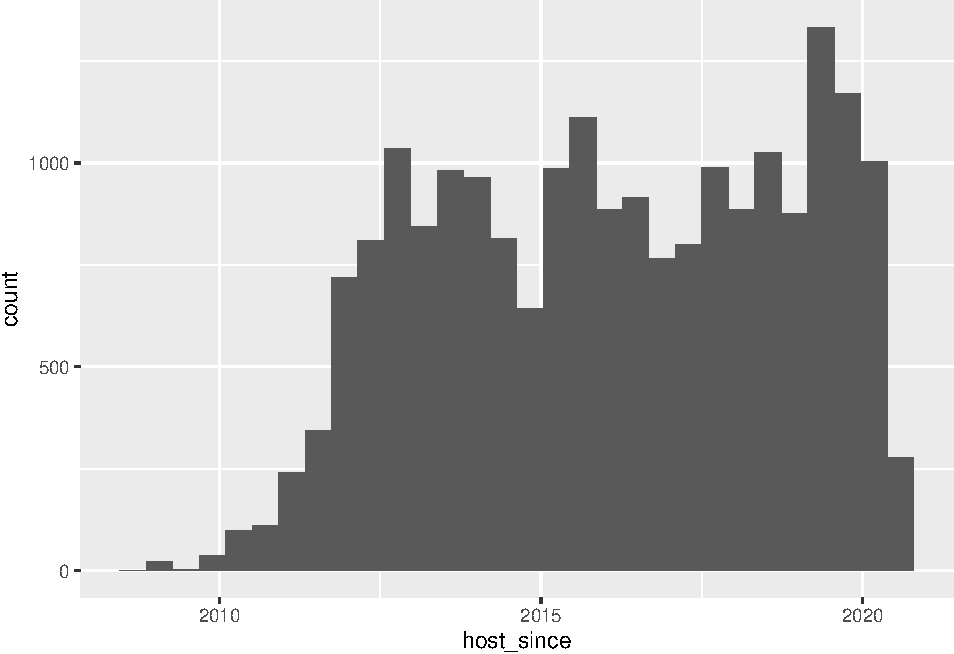
\includegraphics{anal_files/figure-latex/unnamed-chunk-9-1.pdf}

\begin{verbatim}
## [1] "variable  15 : host_response_time"
\end{verbatim}

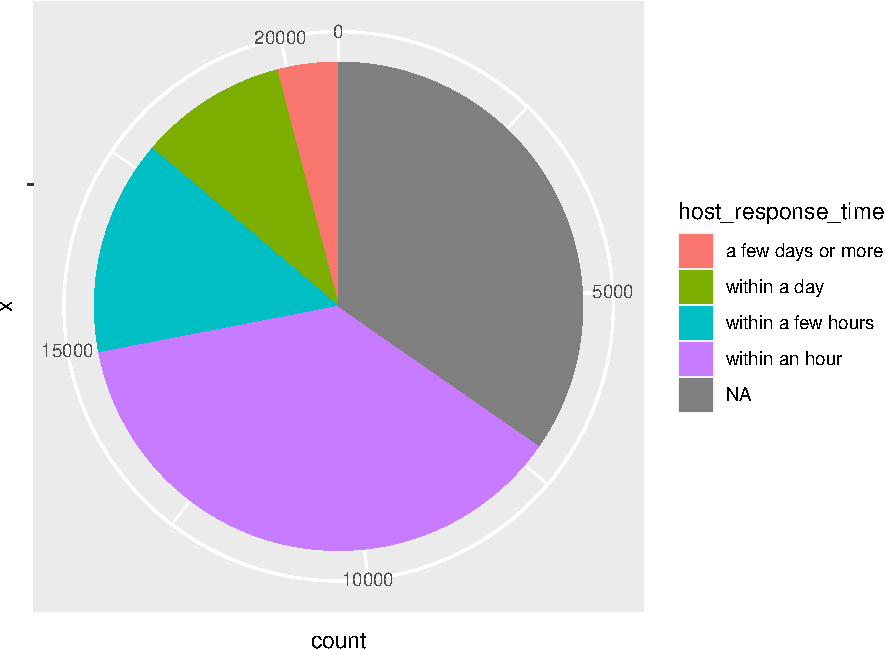
\includegraphics{anal_files/figure-latex/unnamed-chunk-9-2.pdf}
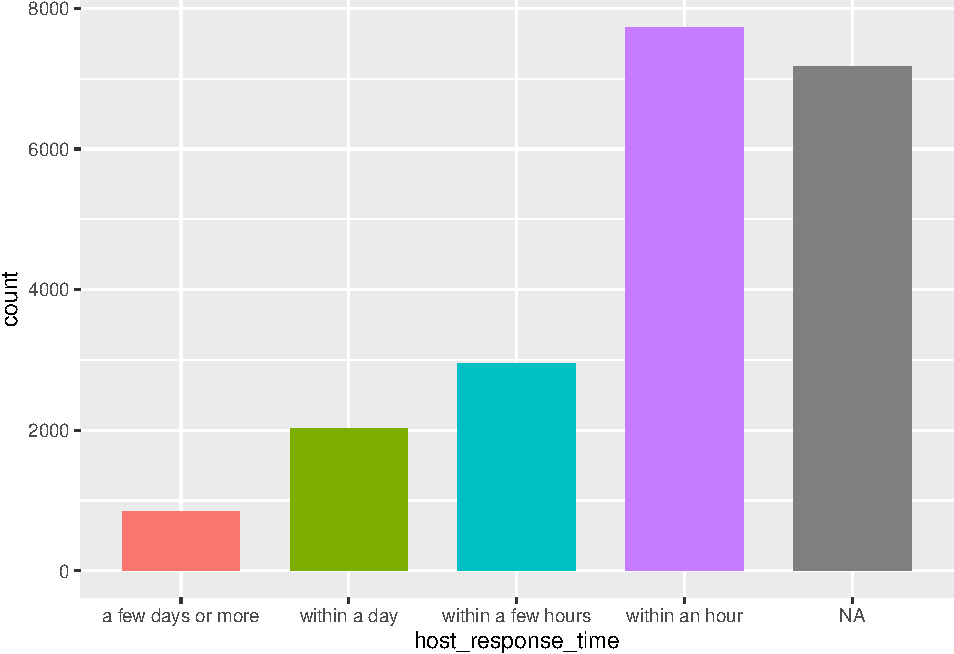
\includegraphics{anal_files/figure-latex/unnamed-chunk-9-3.pdf}

\begin{verbatim}
## [1] "Number of modalities:  5"
## [1] "Frequency table"
## 
## a few days or more       within a day within a few hours     within an hour 
##                843               2018               2946               7722 
##               <NA> 
##               7174 
## [1] "Relative frequency table (proportions)"
## 
## a few days or more       within a day within a few hours     within an hour 
##         0.04071874         0.09747380         0.14229822         0.37298942 
##               <NA> 
##         0.34651983 
## [1] "Frequency table sorted"
## 
##     within an hour               <NA> within a few hours       within a day 
##               7722               7174               2946               2018 
## a few days or more 
##                843 
## [1] "Relative frequency table (proportions) sorted"
## 
##     within an hour               <NA> within a few hours       within a day 
##         0.37298942         0.34651983         0.14229822         0.09747380 
## a few days or more 
##         0.04071874 
## [1] "variable  18 : host_is_superhost"
\end{verbatim}

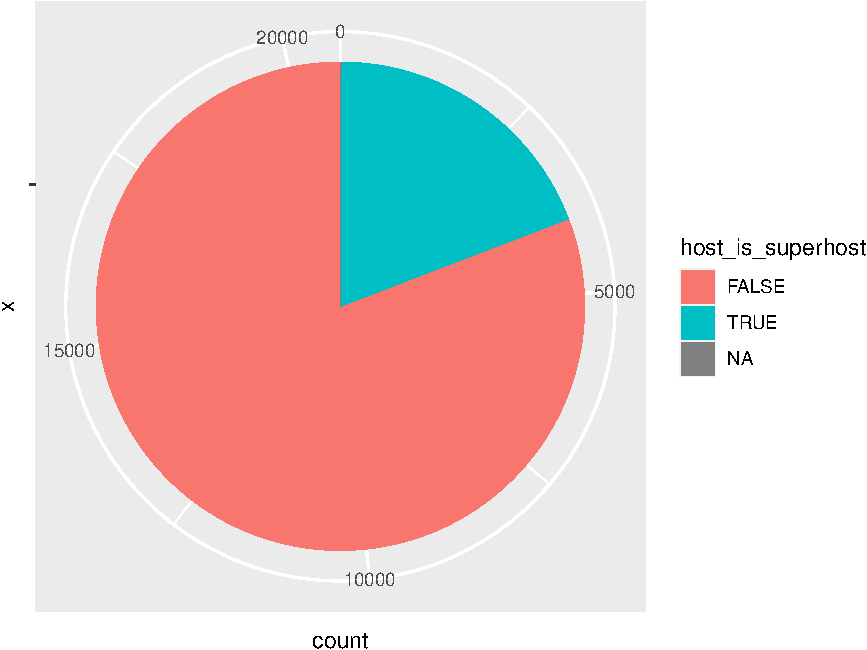
\includegraphics{anal_files/figure-latex/unnamed-chunk-9-4.pdf}
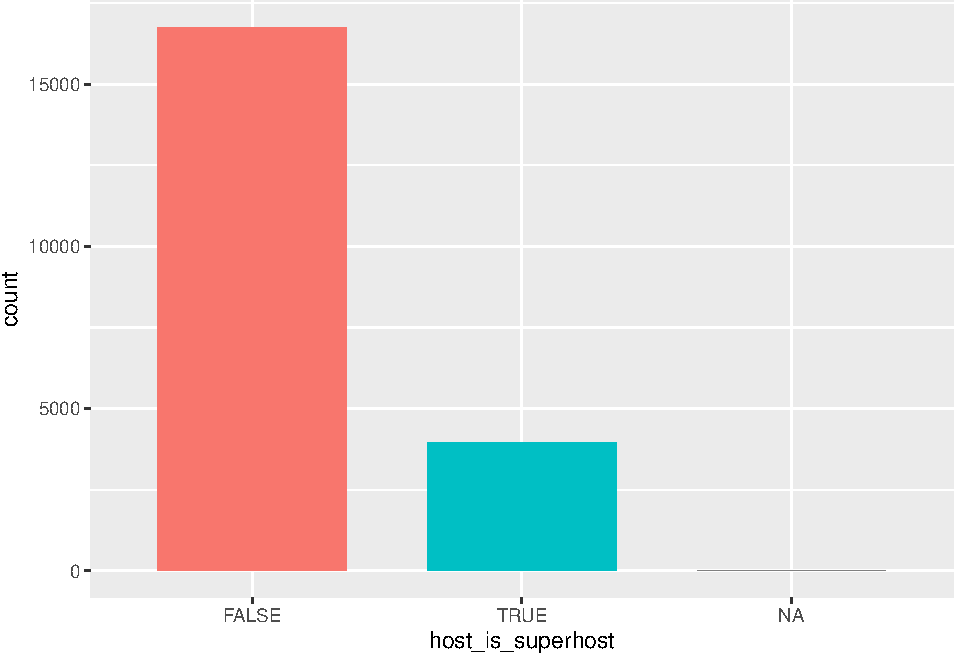
\includegraphics{anal_files/figure-latex/unnamed-chunk-9-5.pdf}

\begin{verbatim}
## [1] "Number of modalities:  3"
## [1] "Frequency table"
## 
## FALSE  TRUE  <NA> 
## 16734  3961     8 
## [1] "Relative frequency table (proportions)"
## 
##        FALSE         TRUE         <NA> 
## 0.8082886538 0.1913249288 0.0003864174 
## [1] "Frequency table sorted"
## 
## FALSE  TRUE  <NA> 
## 16734  3961     8 
## [1] "Relative frequency table (proportions) sorted"
## 
##        FALSE         TRUE         <NA> 
## 0.8082886538 0.1913249288 0.0003864174 
## [1] "variable  22 : host_listings_count"
\end{verbatim}

\begin{verbatim}
## `stat_bin()` using `bins = 30`. Pick better value with `binwidth`.
\end{verbatim}

\begin{verbatim}
## Warning: Removed 8 rows containing non-finite values (stat_bin).
\end{verbatim}

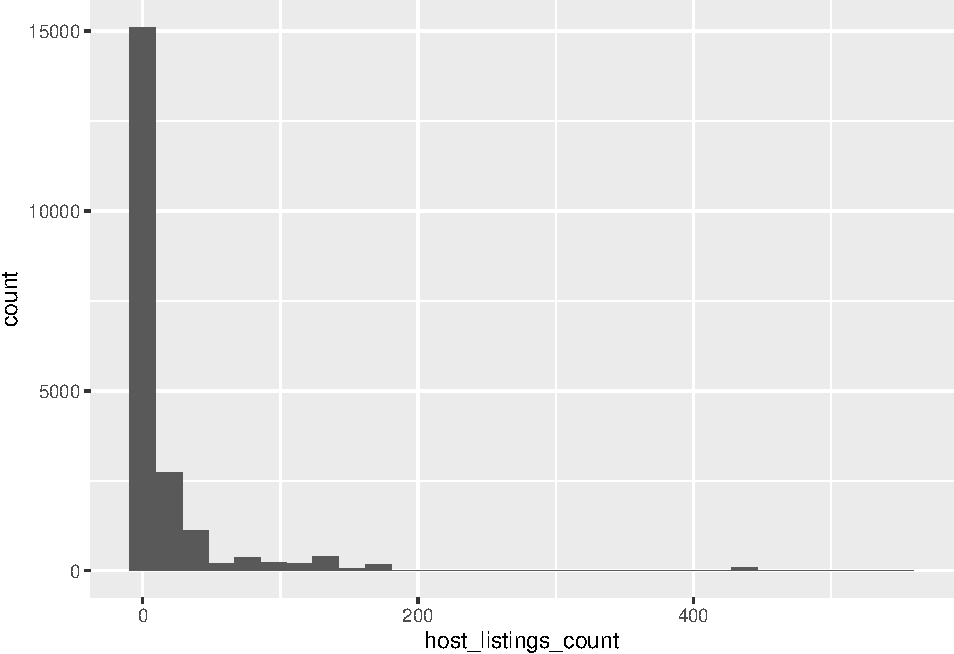
\includegraphics{anal_files/figure-latex/unnamed-chunk-9-6.pdf}

\begin{verbatim}
## Warning: Removed 8 rows containing non-finite values (stat_boxplot).
\end{verbatim}

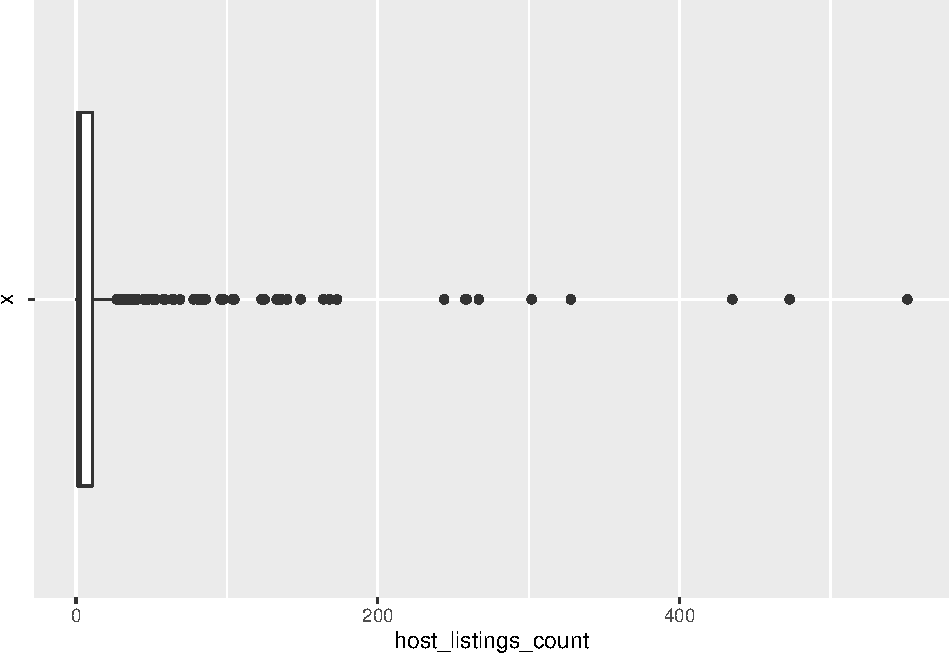
\includegraphics{anal_files/figure-latex/unnamed-chunk-9-7.pdf}

\begin{verbatim}
## [1] "Extended Summary Statistics"
##    Min. 1st Qu.  Median    Mean 3rd Qu.    Max.    NA's 
##    0.00    1.00    2.00   16.81   11.00  551.00       8 
## [1] "sd:  43.3787949847988"
## [1] "vc:  2.58000816835102"
## [1] "variable  25 : host_has_profile_pic"
\end{verbatim}

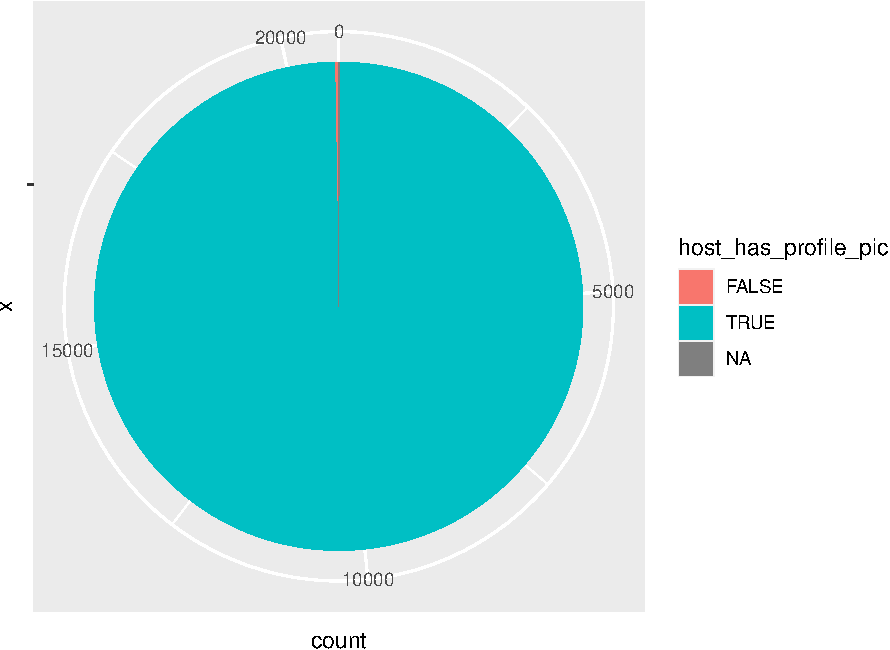
\includegraphics{anal_files/figure-latex/unnamed-chunk-9-8.pdf}
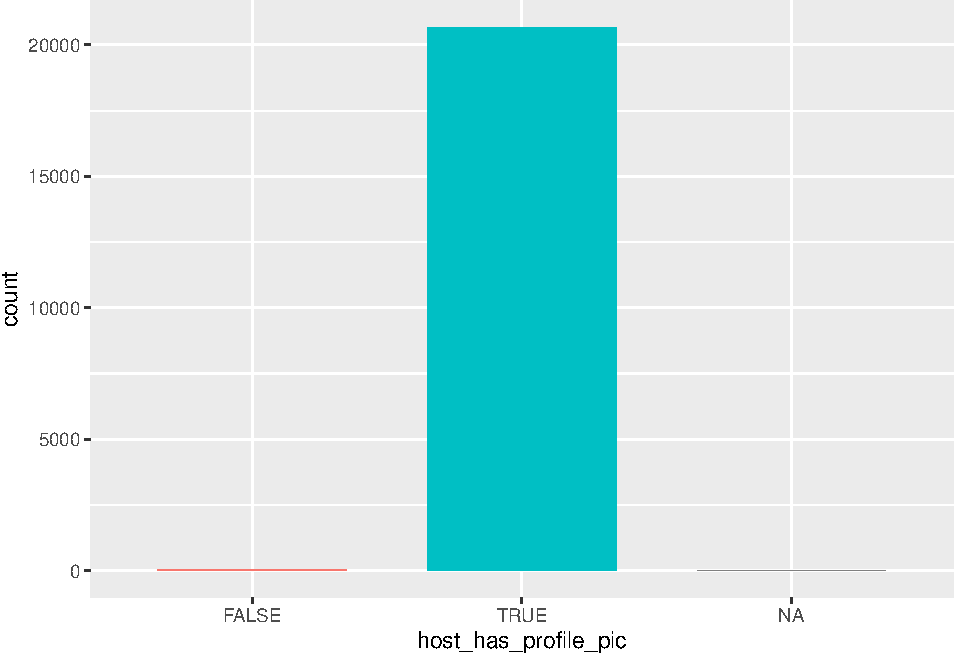
\includegraphics{anal_files/figure-latex/unnamed-chunk-9-9.pdf}

\begin{verbatim}
## [1] "Number of modalities:  3"
## [1] "Frequency table"
## 
## FALSE  TRUE  <NA> 
##    55 20640     8 
## [1] "Relative frequency table (proportions)"
## 
##        FALSE         TRUE         <NA> 
## 0.0026566198 0.9969569628 0.0003864174 
## [1] "Frequency table sorted"
## 
##  TRUE FALSE  <NA> 
## 20640    55     8 
## [1] "Relative frequency table (proportions) sorted"
## 
##         TRUE        FALSE         <NA> 
## 0.9969569628 0.0026566198 0.0003864174 
## [1] "variable  26 : host_identity_verified"
\end{verbatim}

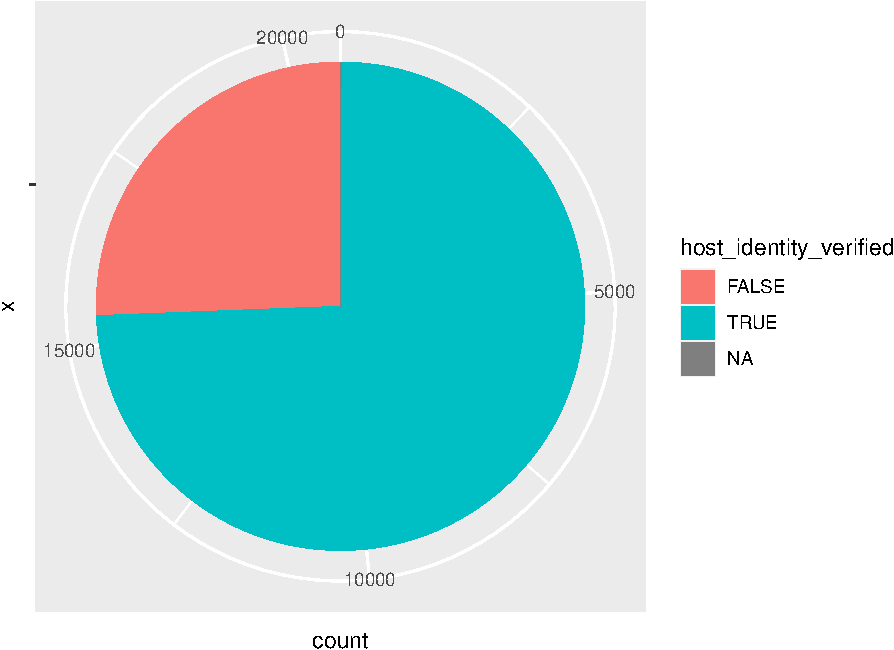
\includegraphics{anal_files/figure-latex/unnamed-chunk-9-10.pdf}
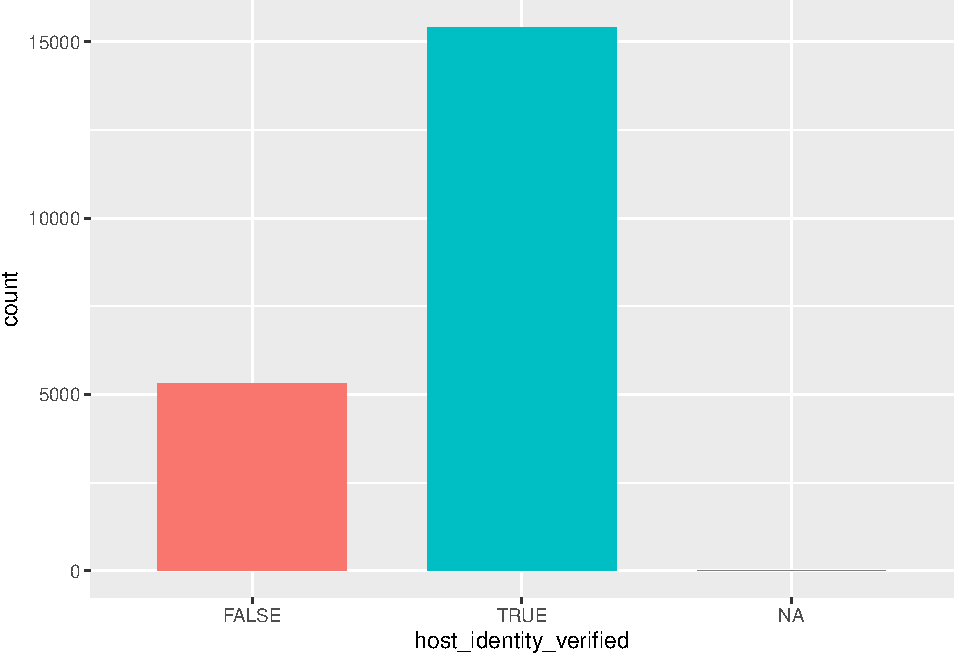
\includegraphics{anal_files/figure-latex/unnamed-chunk-9-11.pdf}

\begin{verbatim}
## [1] "Number of modalities:  3"
## [1] "Frequency table"
## 
## FALSE  TRUE  <NA> 
##  5302 15393     8 
## [1] "Relative frequency table (proportions)"
## 
##        FALSE         TRUE         <NA> 
## 0.2560981500 0.7435154325 0.0003864174 
## [1] "Frequency table sorted"
## 
##  TRUE FALSE  <NA> 
## 15393  5302     8 
## [1] "Relative frequency table (proportions) sorted"
## 
##         TRUE        FALSE         <NA> 
## 0.7435154325 0.2560981500 0.0003864174 
## [1] "variable  29 : neighbourhood_group_cleansed"
\end{verbatim}

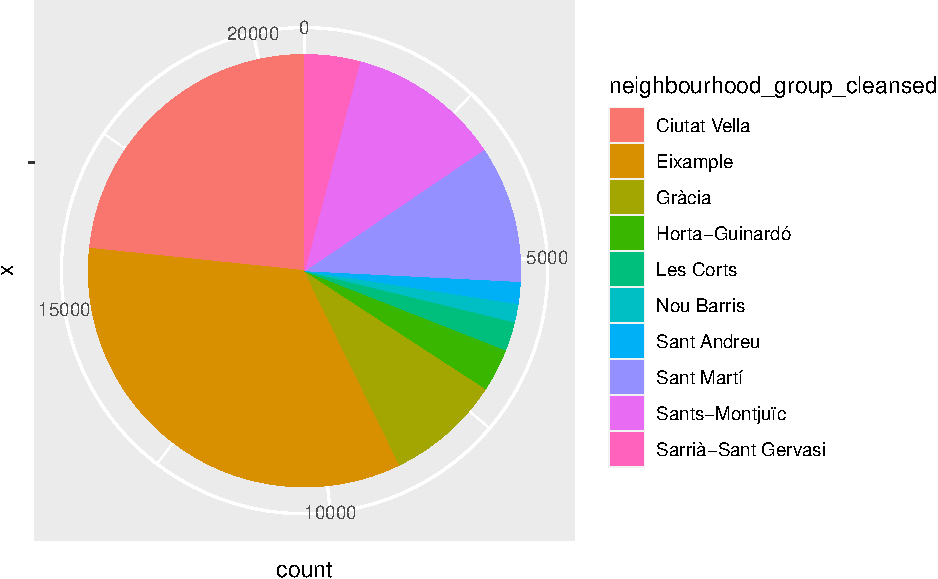
\includegraphics{anal_files/figure-latex/unnamed-chunk-9-12.pdf}
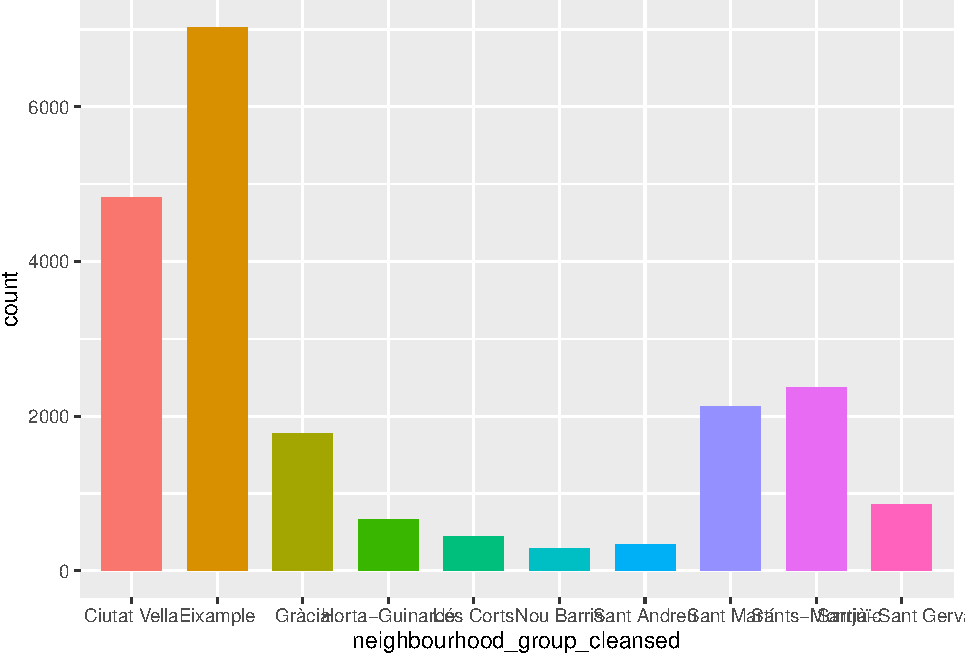
\includegraphics{anal_files/figure-latex/unnamed-chunk-9-13.pdf}

\begin{verbatim}
## [1] "Number of modalities:  10"
## [1] "Frequency table"
## 
##        Ciutat Vella            Eixample              Gràcia      Horta-Guinardó 
##                4834                7020                1773                 665 
##           Les Corts          Nou Barris         Sant Andreu          Sant Martí 
##                 448                 284                 339                2123 
##      Sants-Montjuïc Sarrià-Sant Gervasi 
##                2365                 852 
## [1] "Relative frequency table (proportions)"
## 
##        Ciutat Vella            Eixample              Gràcia      Horta-Guinardó 
##          0.23349273          0.33908129          0.08563976          0.03212095 
##           Les Corts          Nou Barris         Sant Andreu          Sant Martí 
##          0.02163938          0.01371782          0.01637444          0.10254552 
##      Sants-Montjuïc Sarrià-Sant Gervasi 
##          0.11423465          0.04115346 
## [1] "Frequency table sorted"
## 
##            Eixample        Ciutat Vella      Sants-Montjuïc          Sant Martí 
##                7020                4834                2365                2123 
##              Gràcia Sarrià-Sant Gervasi      Horta-Guinardó           Les Corts 
##                1773                 852                 665                 448 
##         Sant Andreu          Nou Barris 
##                 339                 284 
## [1] "Relative frequency table (proportions) sorted"
## 
##            Eixample        Ciutat Vella      Sants-Montjuïc          Sant Martí 
##          0.33908129          0.23349273          0.11423465          0.10254552 
##              Gràcia Sarrià-Sant Gervasi      Horta-Guinardó           Les Corts 
##          0.08563976          0.04115346          0.03212095          0.02163938 
##         Sant Andreu          Nou Barris 
##          0.01637444          0.01371782 
## [1] "variable  33 : room_type"
\end{verbatim}

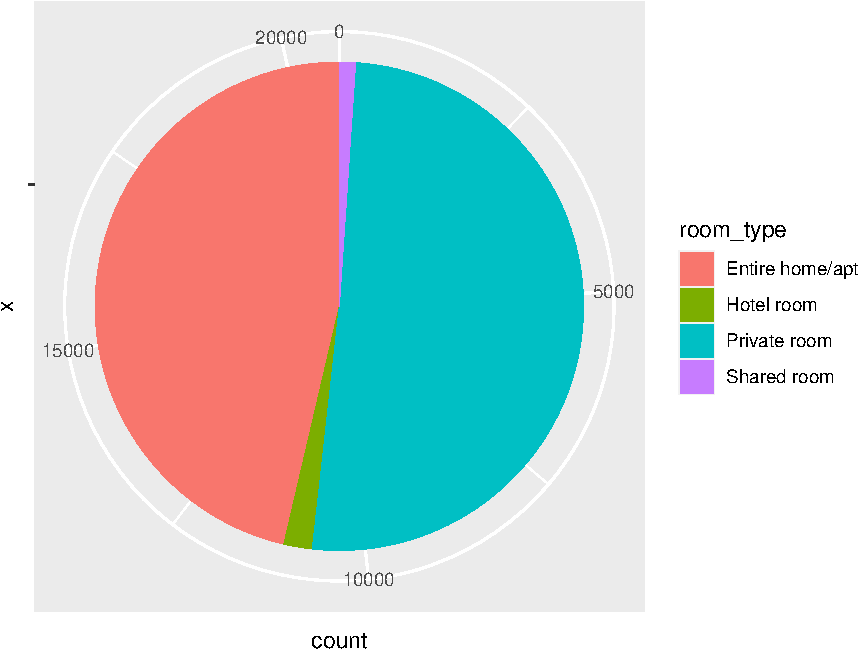
\includegraphics{anal_files/figure-latex/unnamed-chunk-9-14.pdf}
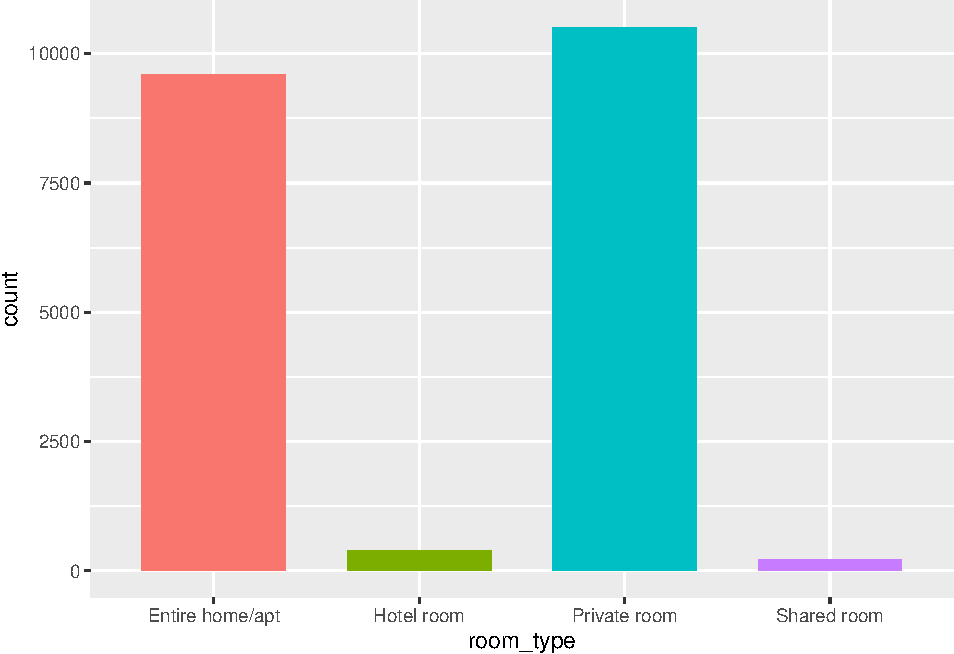
\includegraphics{anal_files/figure-latex/unnamed-chunk-9-15.pdf}

\begin{verbatim}
## [1] "Number of modalities:  4"
## [1] "Frequency table"
## 
## Entire home/apt      Hotel room    Private room     Shared room 
##            9596             390           10497             220 
## [1] "Relative frequency table (proportions)"
## 
## Entire home/apt      Hotel room    Private room     Shared room 
##      0.46350770      0.01883785      0.50702797      0.01062648 
## [1] "Frequency table sorted"
## 
##    Private room Entire home/apt      Hotel room     Shared room 
##           10497            9596             390             220 
## [1] "Relative frequency table (proportions) sorted"
## 
##    Private room Entire home/apt      Hotel room     Shared room 
##      0.50702797      0.46350770      0.01883785      0.01062648 
## [1] "variable  34 : accommodates"
\end{verbatim}

\begin{verbatim}
## `stat_bin()` using `bins = 30`. Pick better value with `binwidth`.
\end{verbatim}

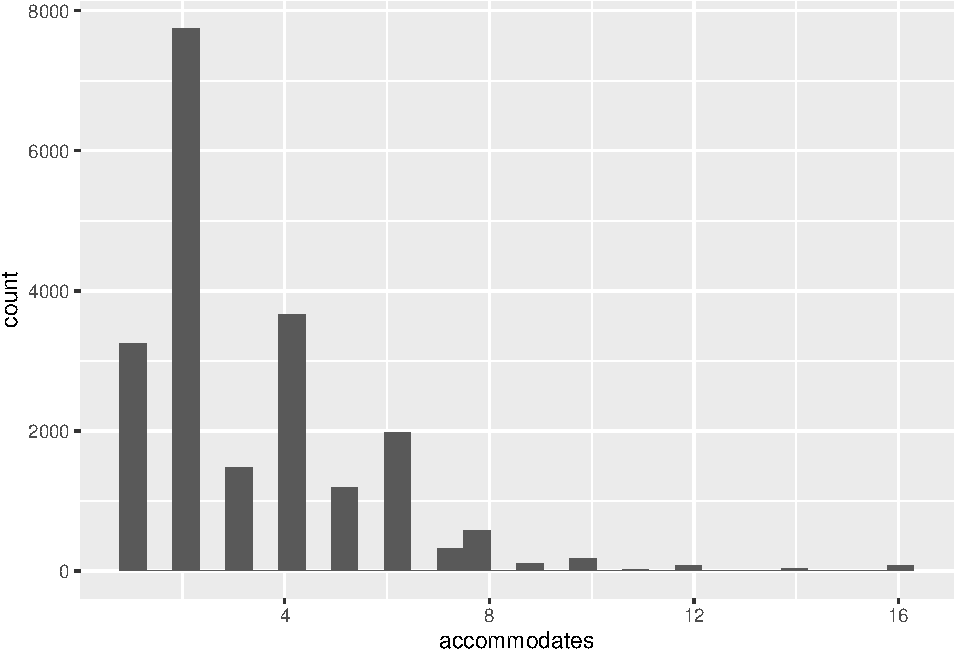
\includegraphics{anal_files/figure-latex/unnamed-chunk-9-16.pdf}
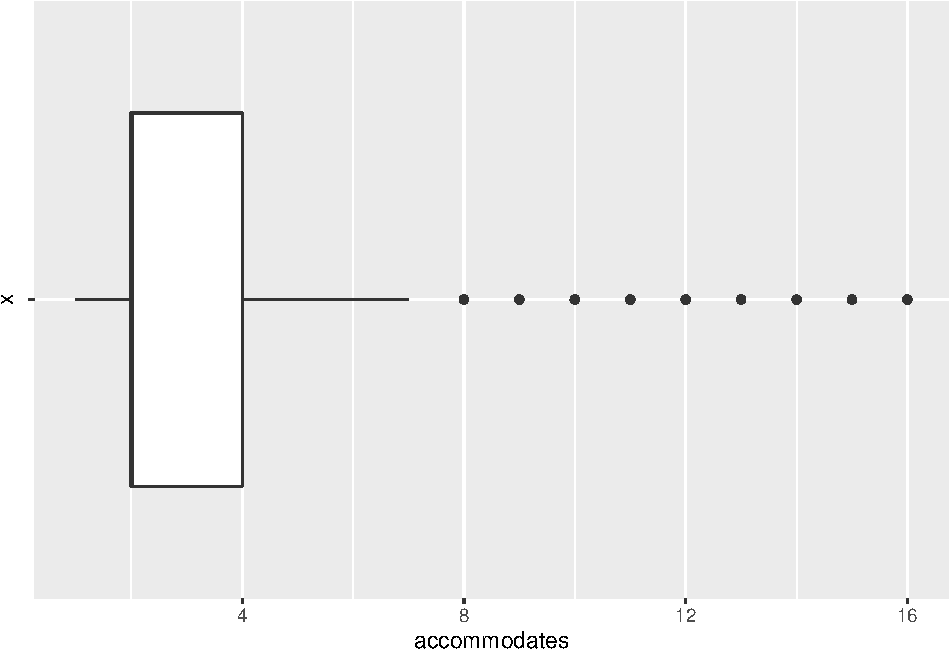
\includegraphics{anal_files/figure-latex/unnamed-chunk-9-17.pdf}

\begin{verbatim}
## [1] "Extended Summary Statistics"
##    Min. 1st Qu.  Median    Mean 3rd Qu.    Max. 
##   1.000   2.000   2.000   3.297   4.000  16.000 
## [1] "sd:  2.23873458185074"
## [1] "vc:  0.679109174464914"
## [1] "variable  37 : bedrooms"
\end{verbatim}

\begin{verbatim}
## `stat_bin()` using `bins = 30`. Pick better value with `binwidth`.
\end{verbatim}

\begin{verbatim}
## Warning: Removed 684 rows containing non-finite values (stat_bin).
\end{verbatim}

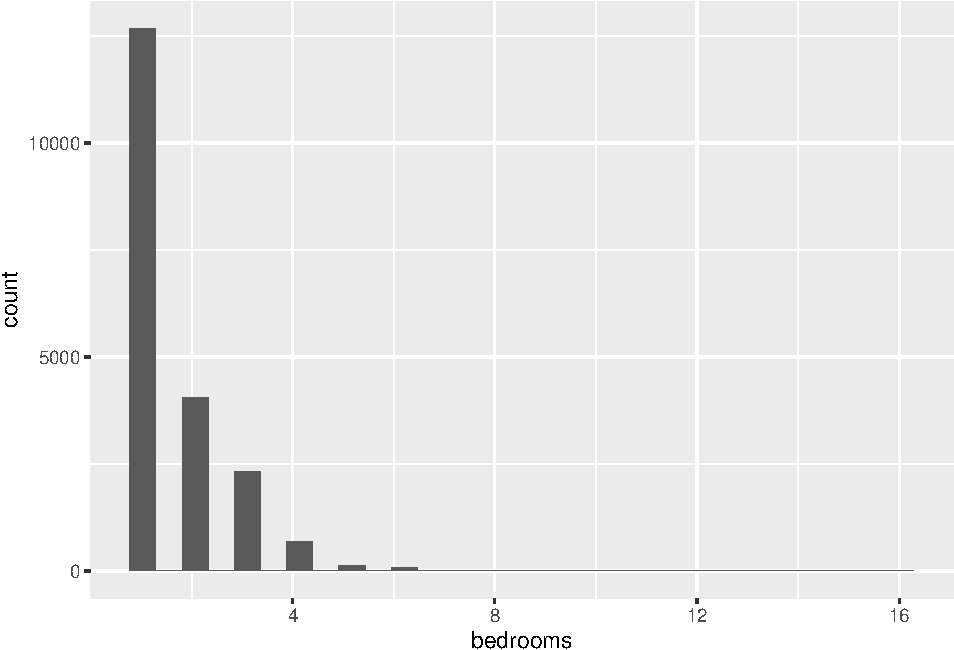
\includegraphics{anal_files/figure-latex/unnamed-chunk-9-18.pdf}

\begin{verbatim}
## Warning: Removed 684 rows containing non-finite values (stat_boxplot).
\end{verbatim}

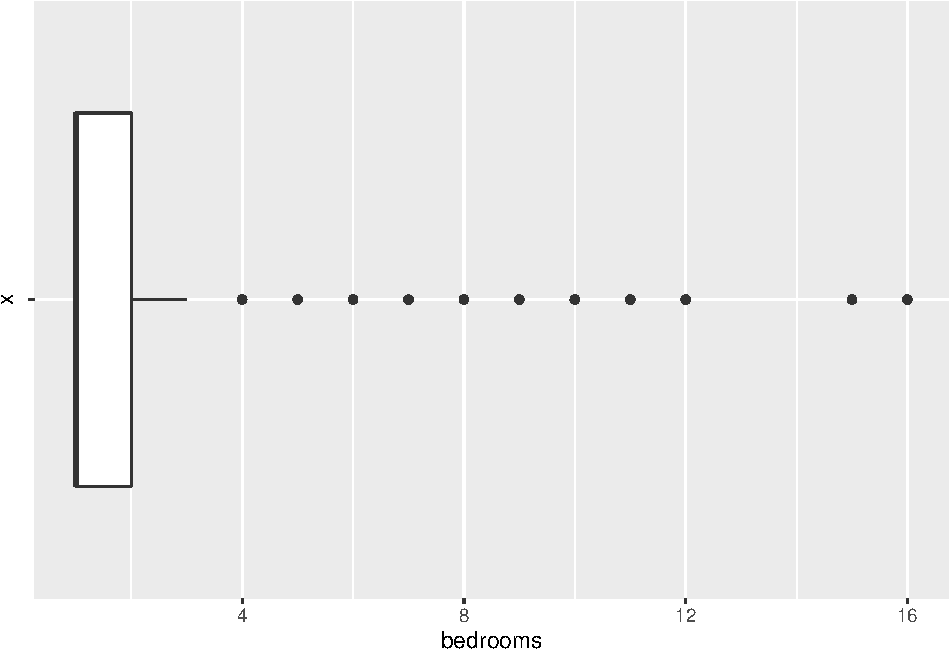
\includegraphics{anal_files/figure-latex/unnamed-chunk-9-19.pdf}

\begin{verbatim}
## [1] "Extended Summary Statistics"
##    Min. 1st Qu.  Median    Mean 3rd Qu.    Max.    NA's 
##   1.000   1.000   1.000   1.604   2.000  16.000     684 
## [1] "sd:  0.991927540847893"
## [1] "vc:  0.618398599864033"
## [1] "variable  38 : beds"
\end{verbatim}

\begin{verbatim}
## `stat_bin()` using `bins = 30`. Pick better value with `binwidth`.
\end{verbatim}

\begin{verbatim}
## Warning: Removed 409 rows containing non-finite values (stat_bin).
\end{verbatim}

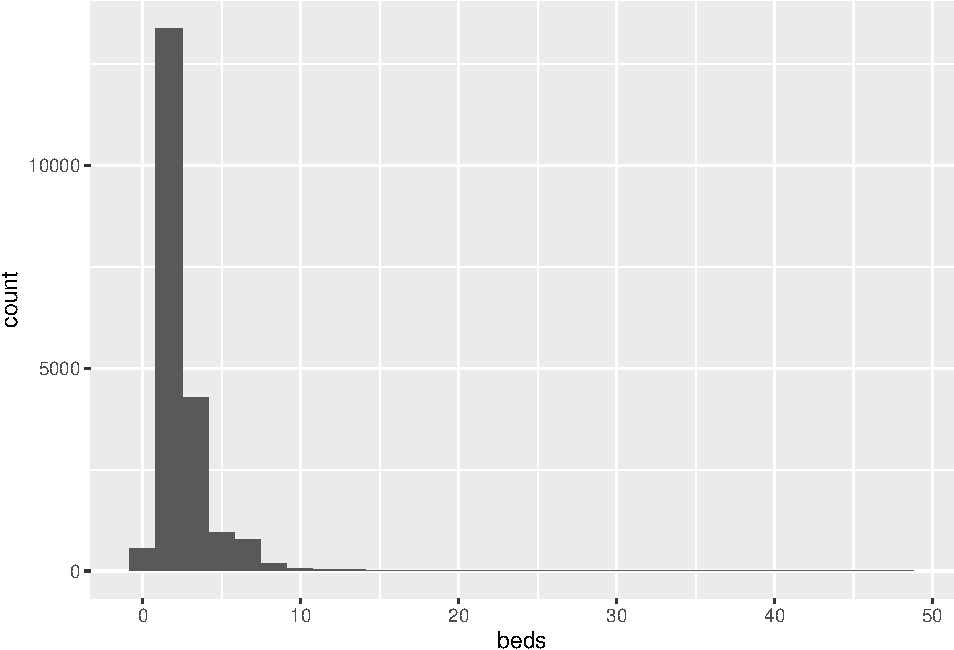
\includegraphics{anal_files/figure-latex/unnamed-chunk-9-20.pdf}

\begin{verbatim}
## Warning: Removed 409 rows containing non-finite values (stat_boxplot).
\end{verbatim}

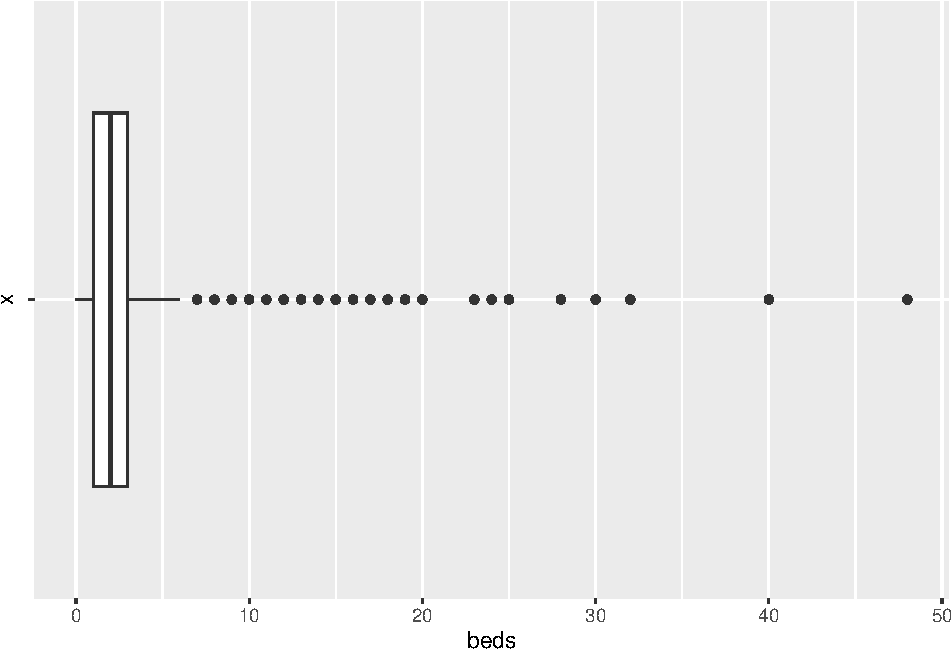
\includegraphics{anal_files/figure-latex/unnamed-chunk-9-21.pdf}

\begin{verbatim}
## [1] "Extended Summary Statistics"
##    Min. 1st Qu.  Median    Mean 3rd Qu.    Max.    NA's 
##   0.000   1.000   2.000   2.233   3.000  48.000     409 
## [1] "sd:  1.9777846692546"
## [1] "vc:  0.885854070446331"
## [1] "variable  40 : price"
\end{verbatim}

\begin{verbatim}
## `stat_bin()` using `bins = 30`. Pick better value with `binwidth`.
\end{verbatim}

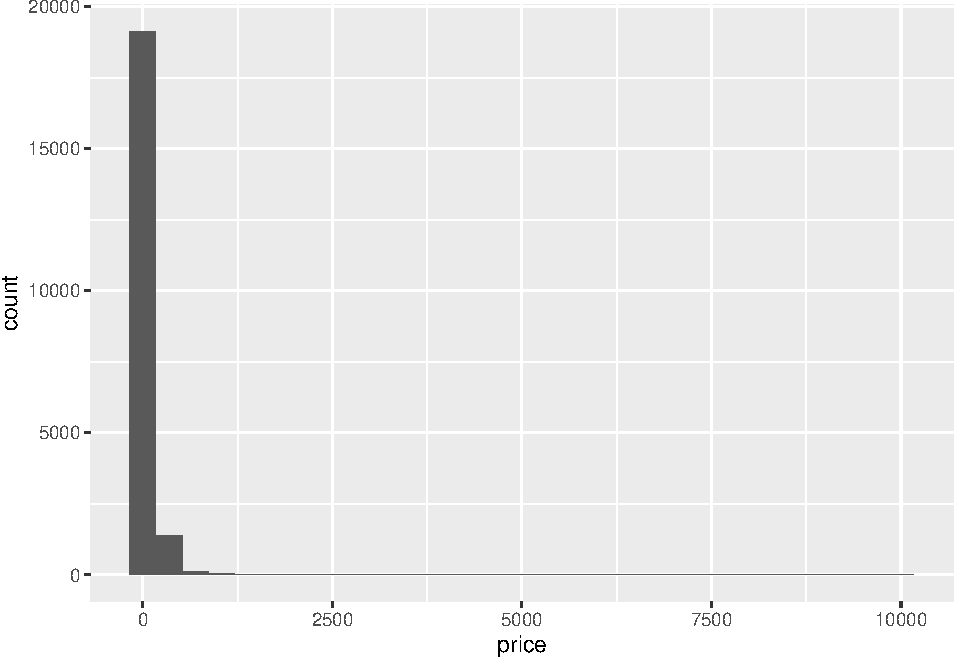
\includegraphics{anal_files/figure-latex/unnamed-chunk-9-22.pdf}
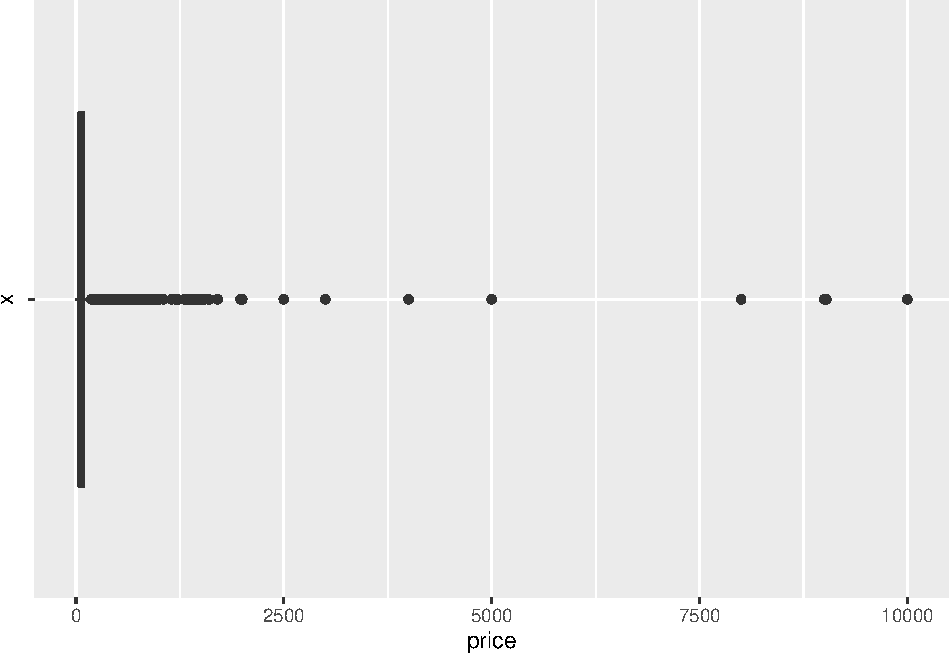
\includegraphics{anal_files/figure-latex/unnamed-chunk-9-23.pdf}

\begin{verbatim}
## [1] "Extended Summary Statistics"
##     Min.  1st Qu.   Median     Mean  3rd Qu.     Max. 
##     0.00    35.00    55.00    86.34    95.00 10000.00 
## [1] "sd:  206.462373757297"
## [1] "vc:  2.39112430629807"
## [1] "variable  47 : minimum_nights_avg_ntm"
\end{verbatim}

\begin{verbatim}
## `stat_bin()` using `bins = 30`. Pick better value with `binwidth`.
\end{verbatim}

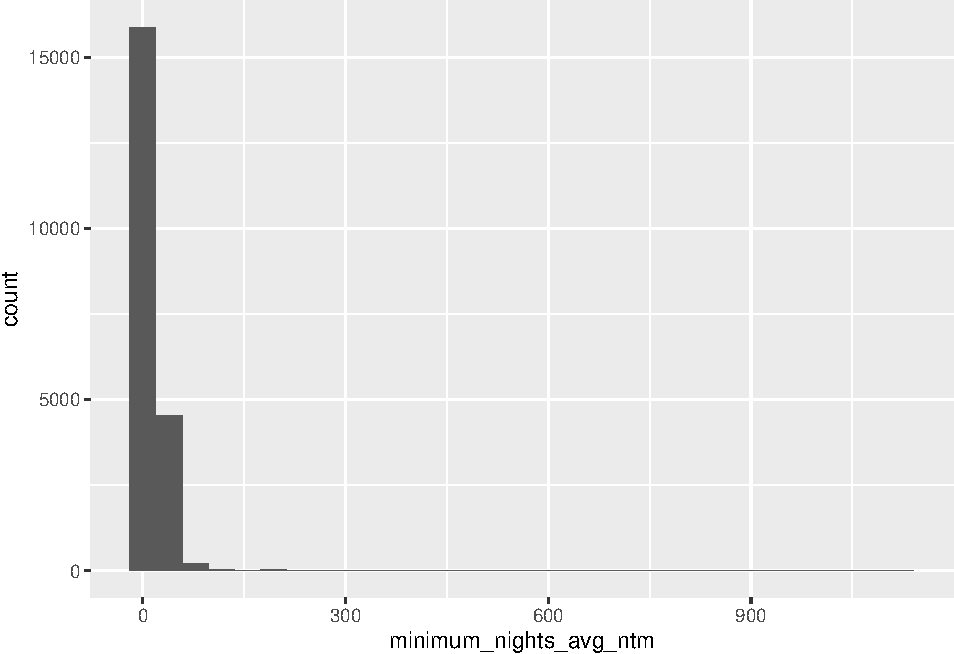
\includegraphics{anal_files/figure-latex/unnamed-chunk-9-24.pdf}
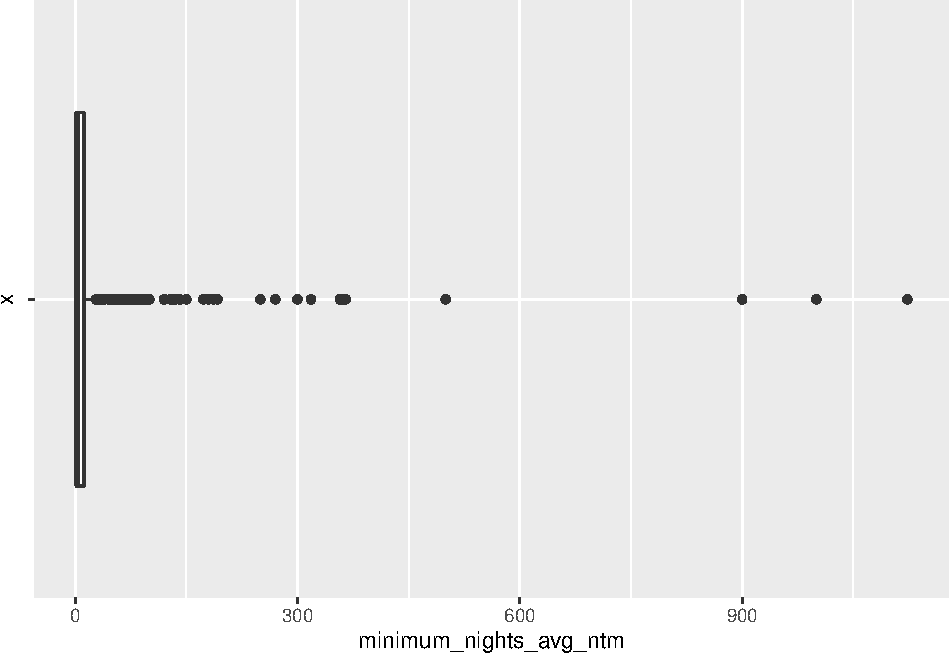
\includegraphics{anal_files/figure-latex/unnamed-chunk-9-25.pdf}

\begin{verbatim}
## [1] "Extended Summary Statistics"
##    Min. 1st Qu.  Median    Mean 3rd Qu.    Max. 
##    1.00    1.40    2.70   10.67   12.10 1123.00 
## [1] "sd:  25.7663823069"
## [1] "vc:  2.41544083534869"
## [1] "variable  48 : maximum_nights_avg_ntm"
\end{verbatim}

\begin{verbatim}
## `stat_bin()` using `bins = 30`. Pick better value with `binwidth`.
\end{verbatim}

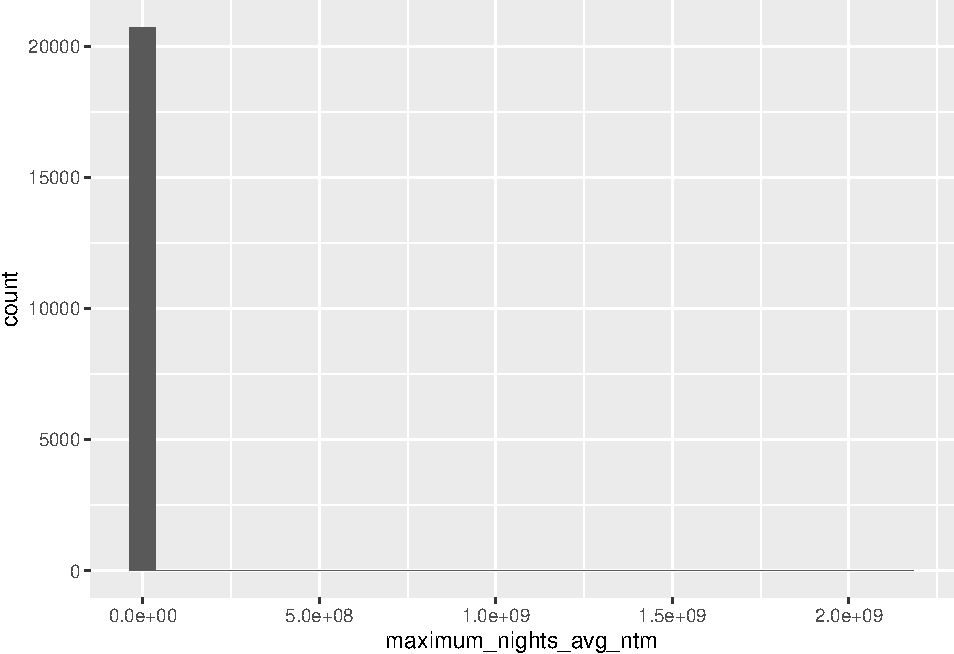
\includegraphics{anal_files/figure-latex/unnamed-chunk-9-26.pdf}
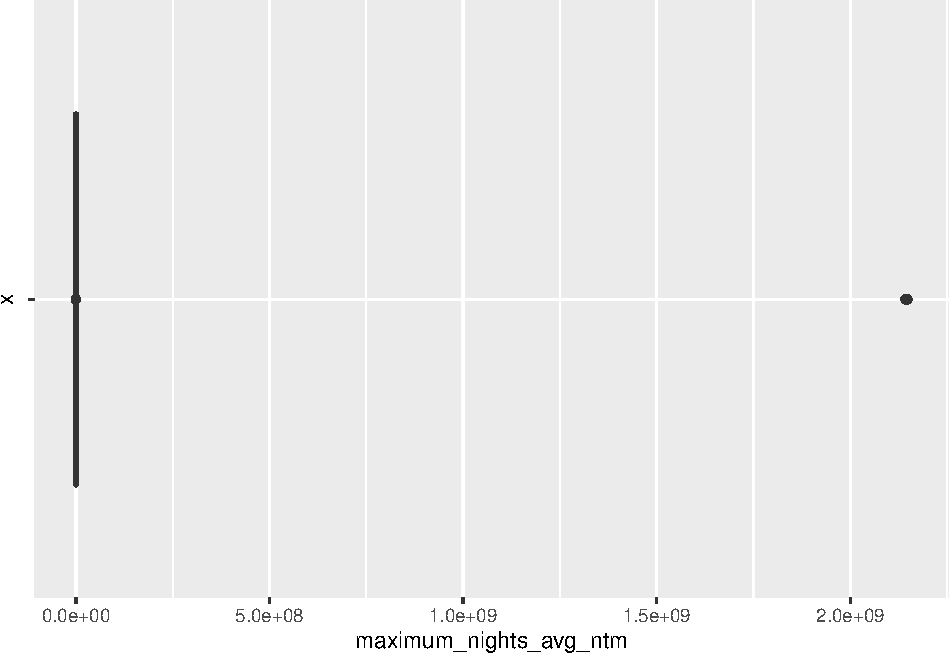
\includegraphics{anal_files/figure-latex/unnamed-chunk-9-27.pdf}

\begin{verbatim}
## [1] "Extended Summary Statistics"
##      Min.   1st Qu.    Median      Mean   3rd Qu.      Max. 
## 1.000e+00 3.300e+02 1.125e+03 3.118e+05 1.125e+03 2.147e+09 
## [1] "sd:  25829740.5605248"
## [1] "vc:  82.8528295497124"
## [1] "variable  51 : availability_30"
\end{verbatim}

\begin{verbatim}
## `stat_bin()` using `bins = 30`. Pick better value with `binwidth`.
\end{verbatim}

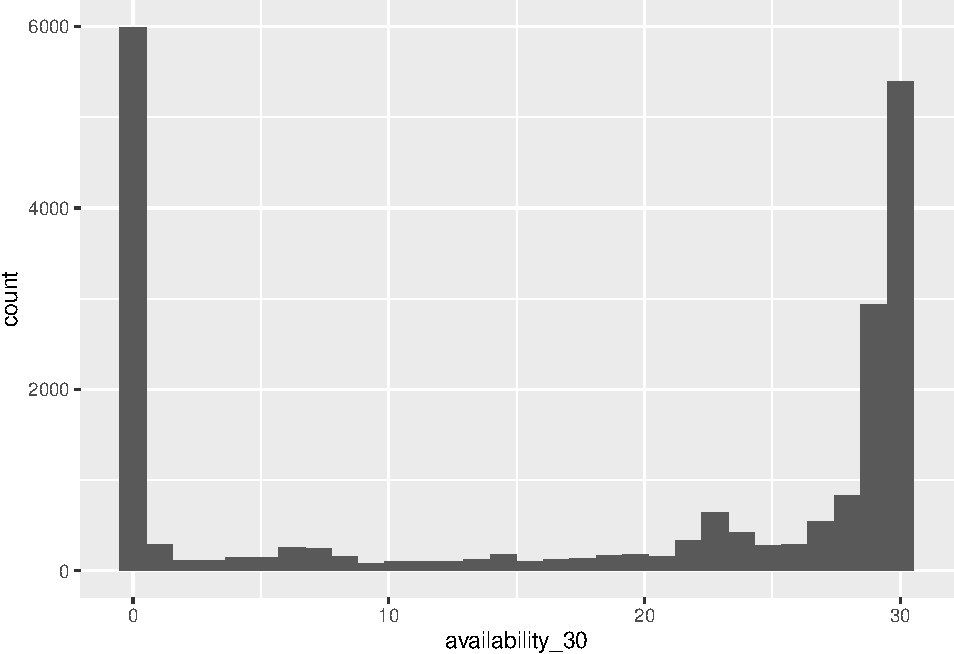
\includegraphics{anal_files/figure-latex/unnamed-chunk-9-28.pdf}
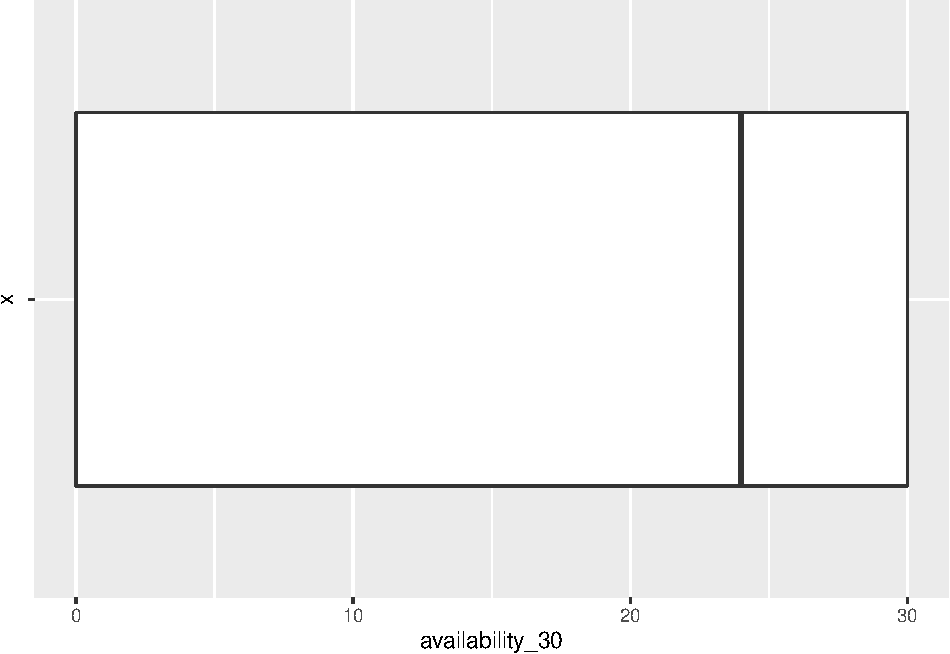
\includegraphics{anal_files/figure-latex/unnamed-chunk-9-29.pdf}

\begin{verbatim}
## [1] "Extended Summary Statistics"
##    Min. 1st Qu.  Median    Mean 3rd Qu.    Max. 
##    0.00    0.00   24.00   17.55   30.00   30.00 
## [1] "sd:  13.1256857815973"
## [1] "vc:  0.748066313023828"
## [1] "variable  52 : availability_60"
\end{verbatim}

\begin{verbatim}
## `stat_bin()` using `bins = 30`. Pick better value with `binwidth`.
\end{verbatim}

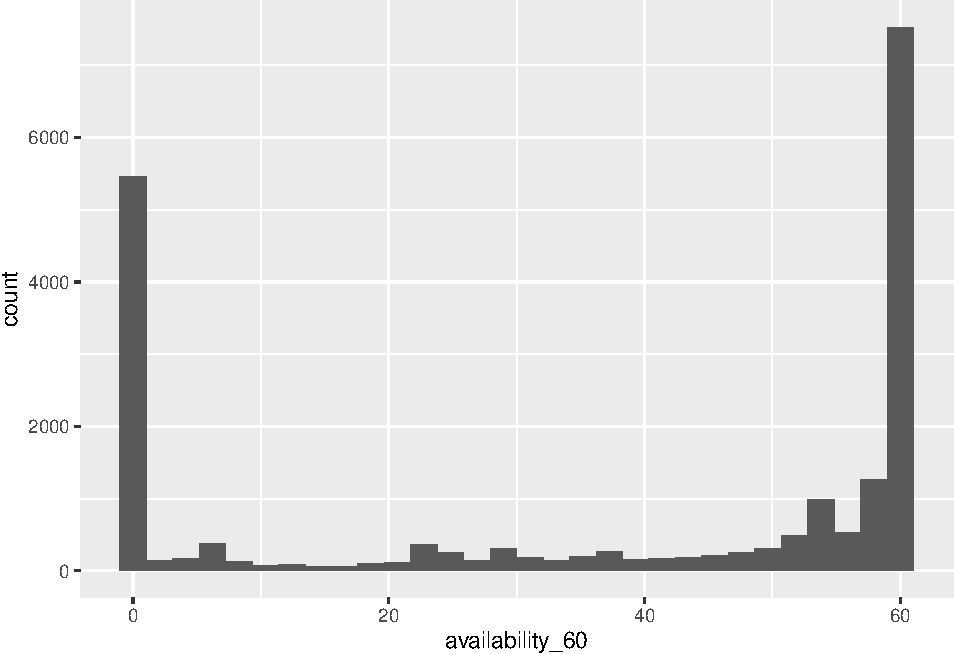
\includegraphics{anal_files/figure-latex/unnamed-chunk-9-30.pdf}
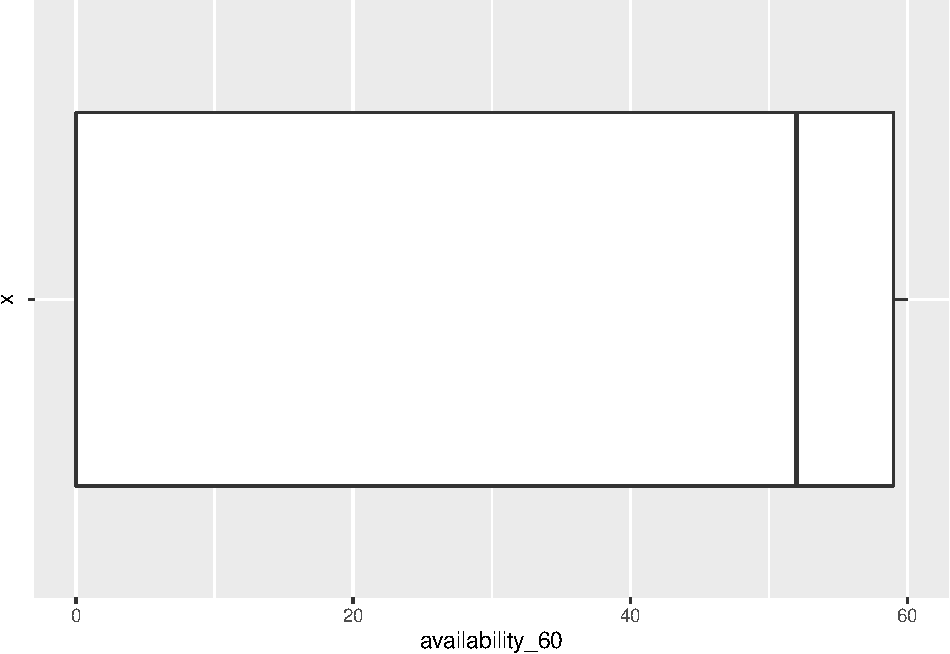
\includegraphics{anal_files/figure-latex/unnamed-chunk-9-31.pdf}

\begin{verbatim}
## [1] "Extended Summary Statistics"
##    Min. 1st Qu.  Median    Mean 3rd Qu.    Max. 
##    0.00    0.00   52.00   36.43   59.00   60.00 
## [1] "sd:  25.7246770560561"
## [1] "vc:  0.706174828708438"
## [1] "variable  53 : availability_90"
\end{verbatim}

\begin{verbatim}
## `stat_bin()` using `bins = 30`. Pick better value with `binwidth`.
\end{verbatim}

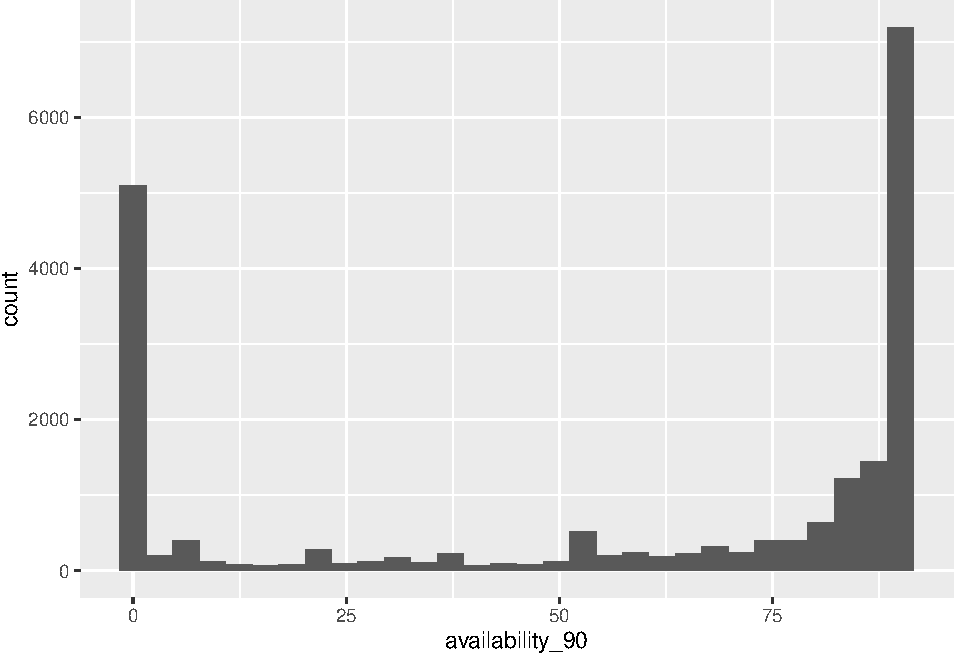
\includegraphics{anal_files/figure-latex/unnamed-chunk-9-32.pdf}
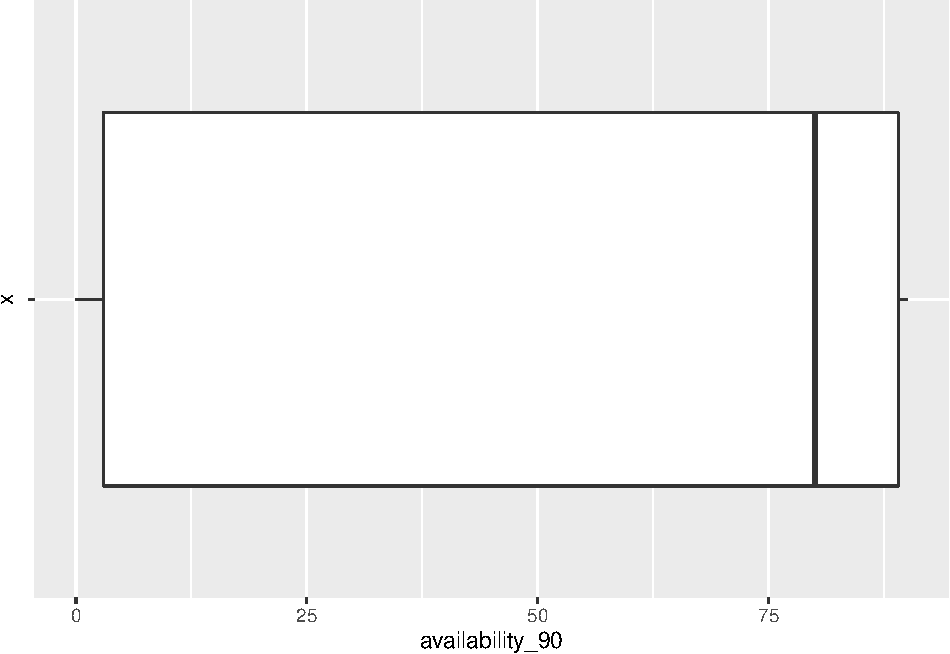
\includegraphics{anal_files/figure-latex/unnamed-chunk-9-33.pdf}

\begin{verbatim}
## [1] "Extended Summary Statistics"
##    Min. 1st Qu.  Median    Mean 3rd Qu.    Max. 
##    0.00    3.00   80.00   56.01   89.00   90.00 
## [1] "sd:  38.3144345211077"
## [1] "vc:  0.684065373969981"
## [1] "variable  54 : availability_365"
\end{verbatim}

\begin{verbatim}
## `stat_bin()` using `bins = 30`. Pick better value with `binwidth`.
\end{verbatim}

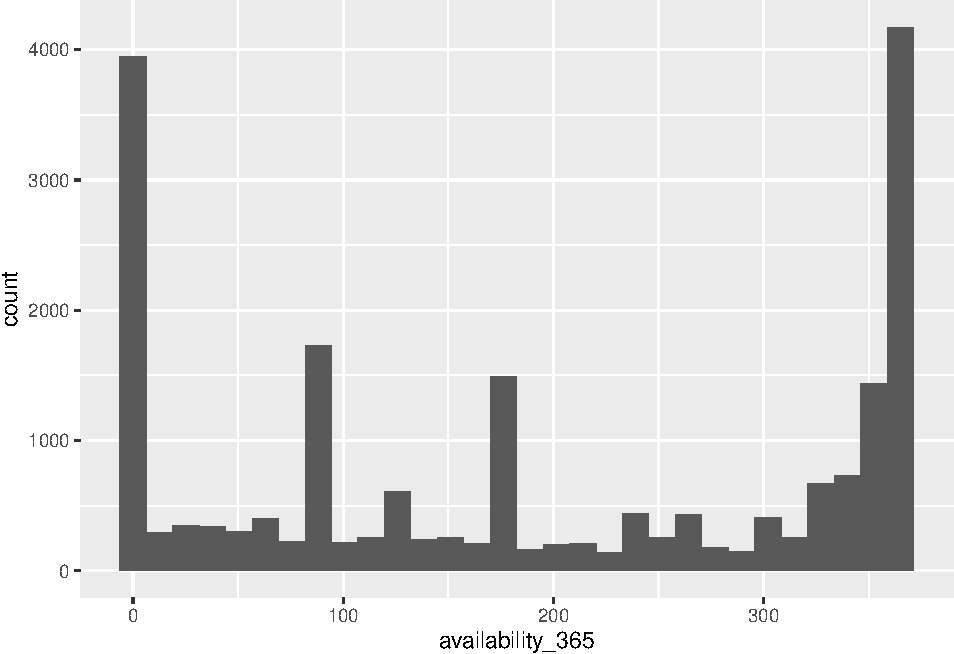
\includegraphics{anal_files/figure-latex/unnamed-chunk-9-34.pdf}
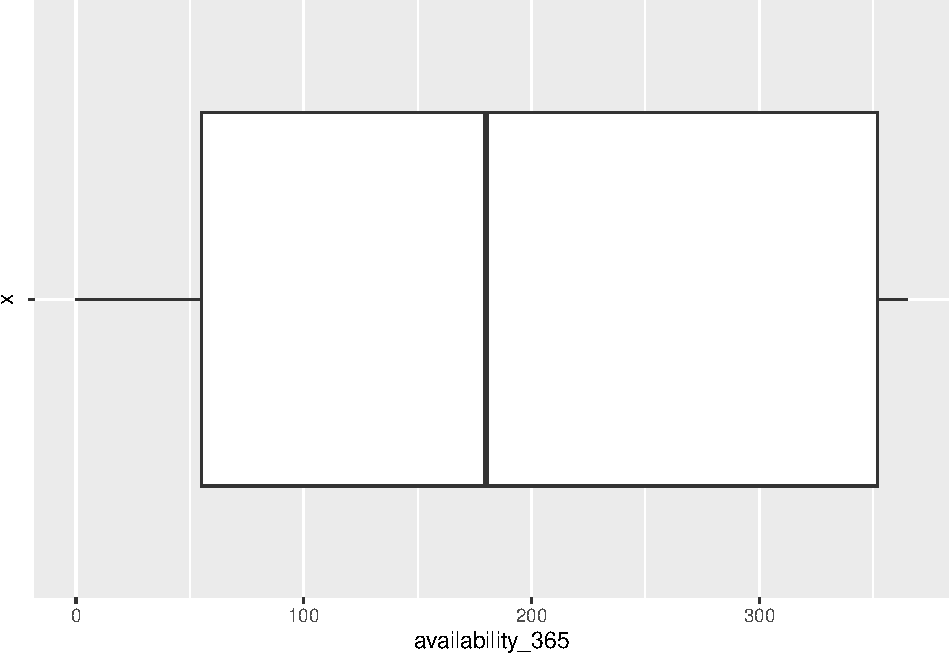
\includegraphics{anal_files/figure-latex/unnamed-chunk-9-35.pdf}

\begin{verbatim}
## [1] "Extended Summary Statistics"
##    Min. 1st Qu.  Median    Mean 3rd Qu.    Max. 
##     0.0    55.0   180.0   191.3   352.0   365.0 
## [1] "sd:  142.34942312352"
## [1] "vc:  0.744162184889913"
## [1] "variable  56 : number_of_reviews"
\end{verbatim}

\begin{verbatim}
## `stat_bin()` using `bins = 30`. Pick better value with `binwidth`.
\end{verbatim}

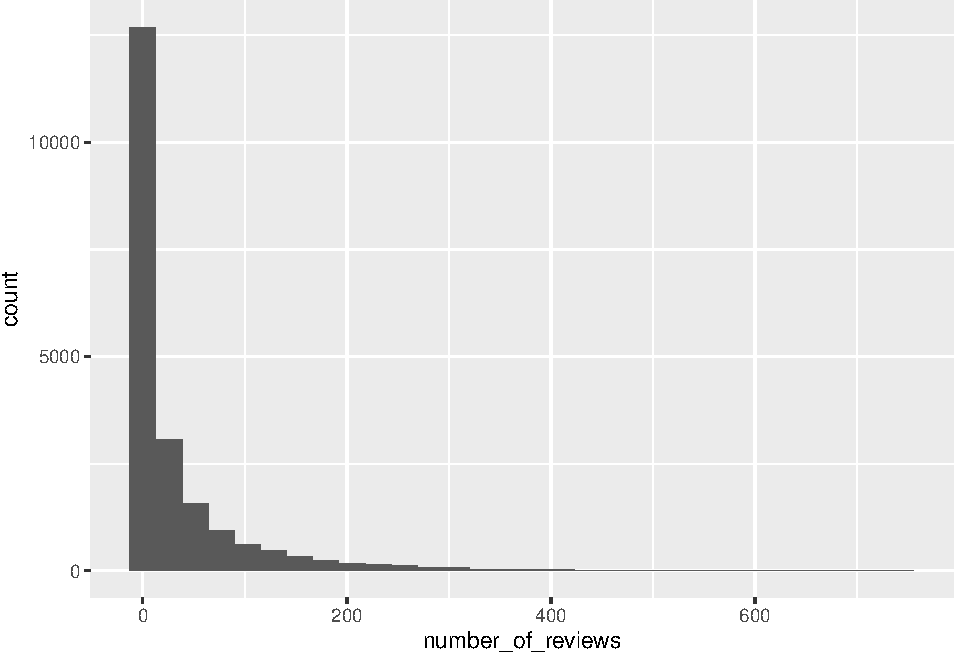
\includegraphics{anal_files/figure-latex/unnamed-chunk-9-36.pdf}
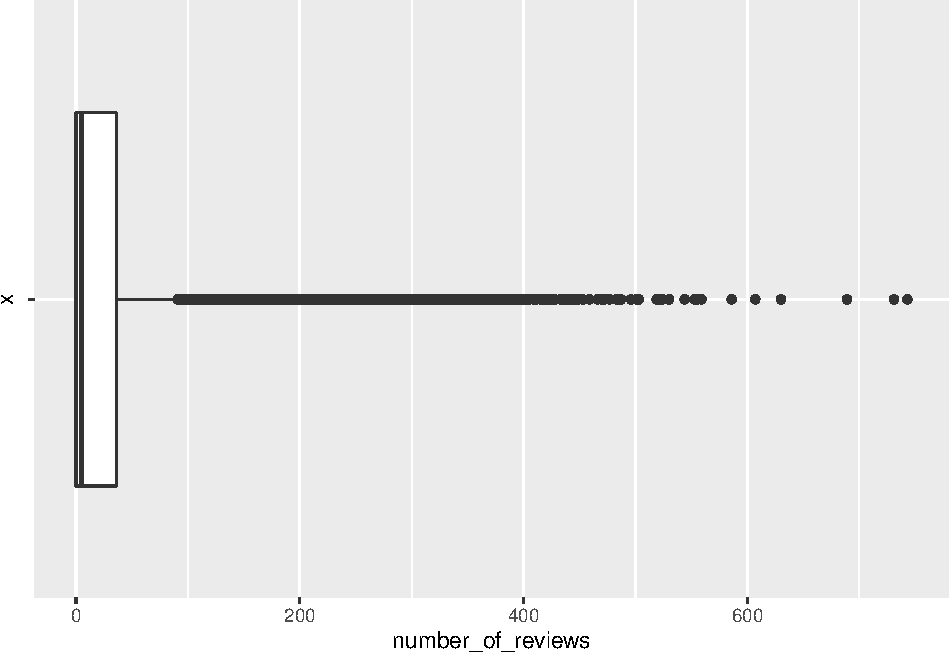
\includegraphics{anal_files/figure-latex/unnamed-chunk-9-37.pdf}

\begin{verbatim}
## [1] "Extended Summary Statistics"
##    Min. 1st Qu.  Median    Mean 3rd Qu.    Max. 
##     0.0     0.0     5.0    33.1    36.0   743.0 
## [1] "sd:  63.3189933063887"
## [1] "vc:  1.91281341970952"
## [1] "variable  57 : number_of_reviews_ltm"
\end{verbatim}

\begin{verbatim}
## `stat_bin()` using `bins = 30`. Pick better value with `binwidth`.
\end{verbatim}

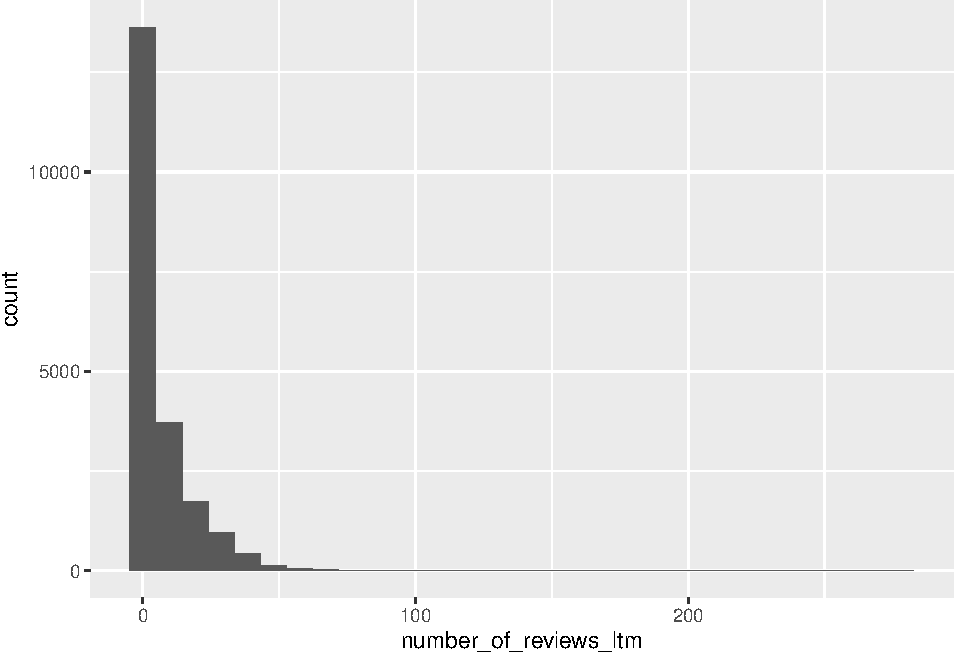
\includegraphics{anal_files/figure-latex/unnamed-chunk-9-38.pdf}
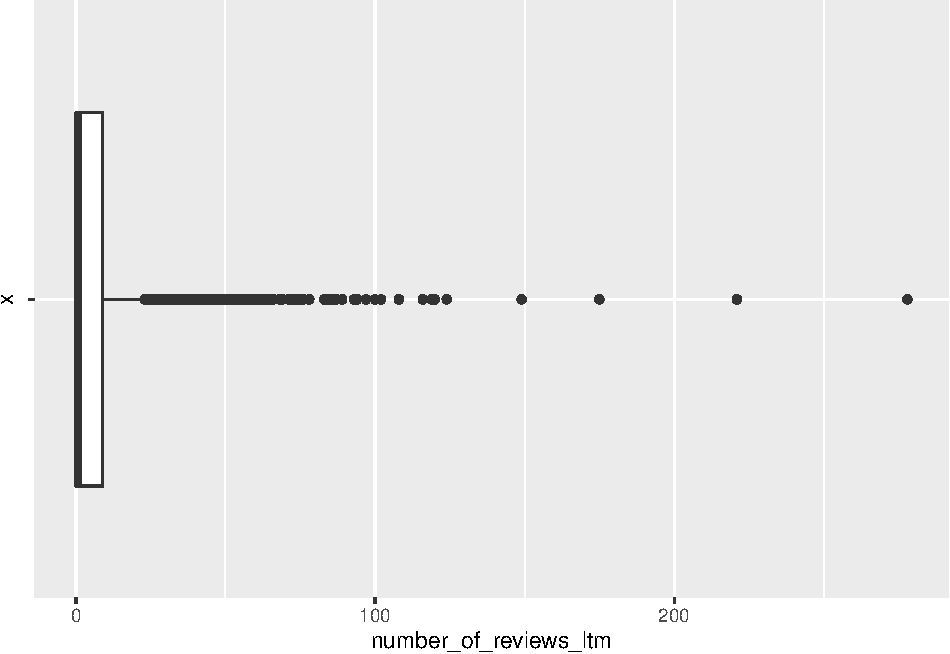
\includegraphics{anal_files/figure-latex/unnamed-chunk-9-39.pdf}

\begin{verbatim}
## [1] "Extended Summary Statistics"
##    Min. 1st Qu.  Median    Mean 3rd Qu.    Max. 
##   0.000   0.000   1.000   6.401   9.000 278.000 
## [1] "sd:  11.1280843101846"
## [1] "vc:  1.73849026164919"
## [1] "variable  58 : number_of_reviews_l30d"
\end{verbatim}

\begin{verbatim}
## `stat_bin()` using `bins = 30`. Pick better value with `binwidth`.
\end{verbatim}

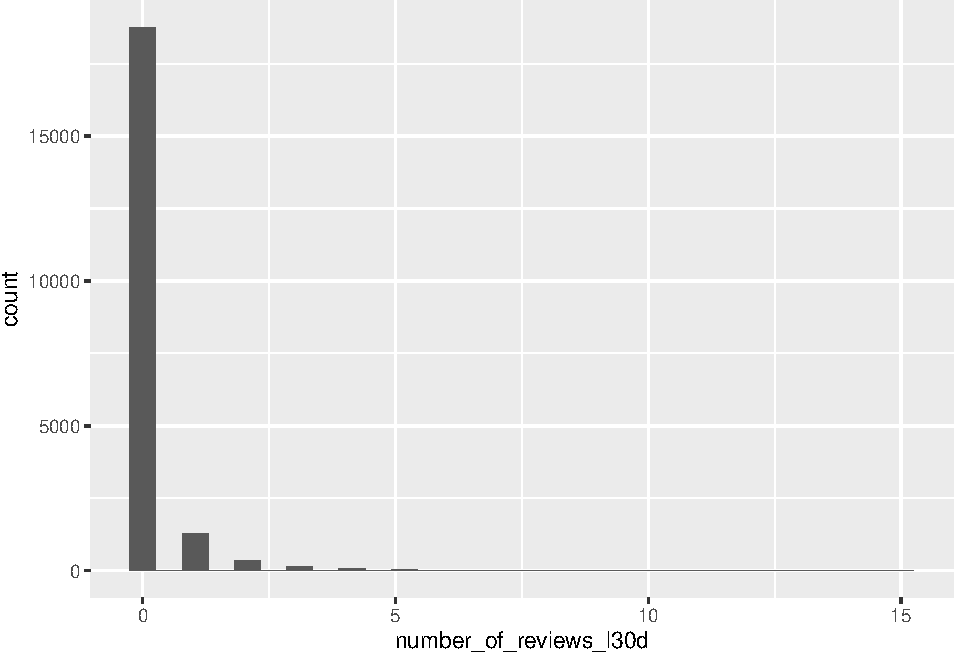
\includegraphics{anal_files/figure-latex/unnamed-chunk-9-40.pdf}
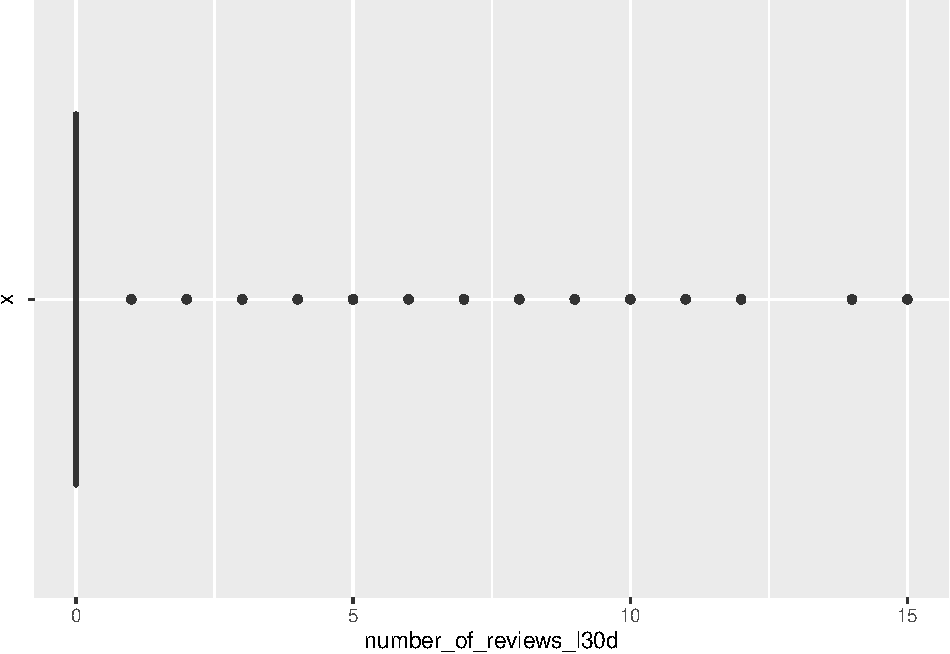
\includegraphics{anal_files/figure-latex/unnamed-chunk-9-41.pdf}

\begin{verbatim}
## [1] "Extended Summary Statistics"
##    Min. 1st Qu.  Median    Mean 3rd Qu.    Max. 
##  0.0000  0.0000  0.0000  0.1621  0.0000 15.0000 
## [1] "sd:  0.661615277330759"
## [1] "vc:  4.0814723142368"
## [1] "variable  61 : review_scores_rating"
\end{verbatim}

\begin{verbatim}
## `stat_bin()` using `bins = 30`. Pick better value with `binwidth`.
\end{verbatim}

\begin{verbatim}
## Warning: Removed 5971 rows containing non-finite values (stat_bin).
\end{verbatim}

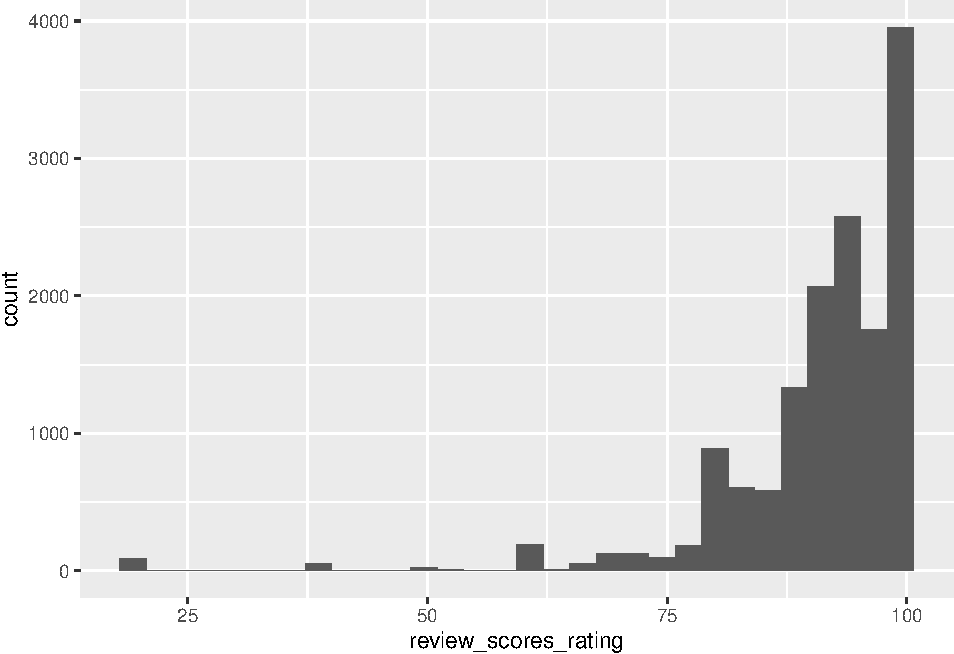
\includegraphics{anal_files/figure-latex/unnamed-chunk-9-42.pdf}

\begin{verbatim}
## Warning: Removed 5971 rows containing non-finite values (stat_boxplot).
\end{verbatim}

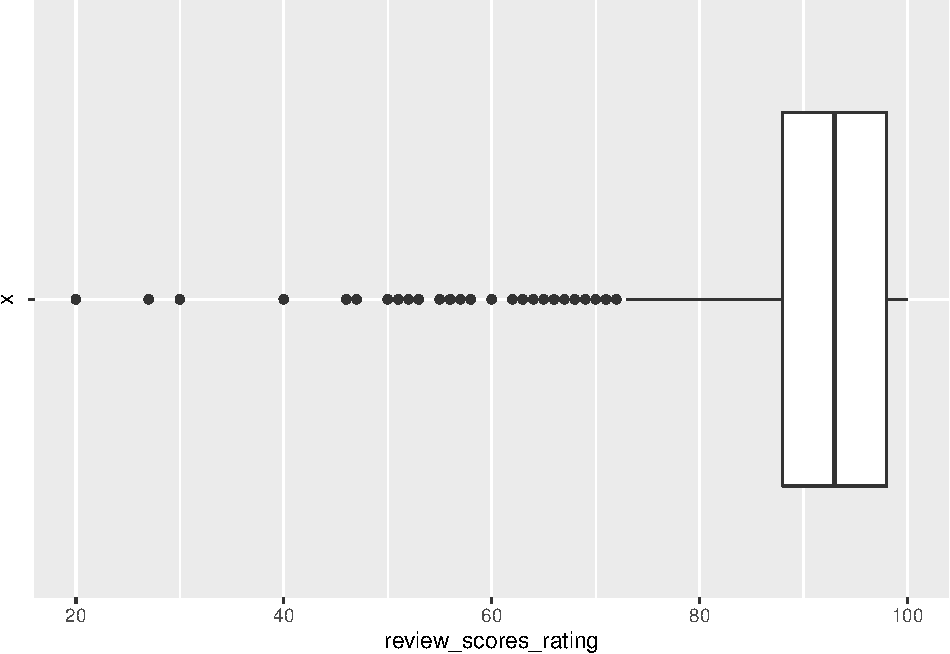
\includegraphics{anal_files/figure-latex/unnamed-chunk-9-43.pdf}

\begin{verbatim}
## [1] "Extended Summary Statistics"
##    Min. 1st Qu.  Median    Mean 3rd Qu.    Max.    NA's 
##   20.00   88.00   93.00   91.08   98.00  100.00    5971 
## [1] "sd:  10.4587403853611"
## [1] "vc:  0.114830482428774"
## [1] "variable  62 : review_scores_accuracy"
\end{verbatim}

\begin{verbatim}
## `stat_bin()` using `bins = 30`. Pick better value with `binwidth`.
\end{verbatim}

\begin{verbatim}
## Warning: Removed 5982 rows containing non-finite values (stat_bin).
\end{verbatim}

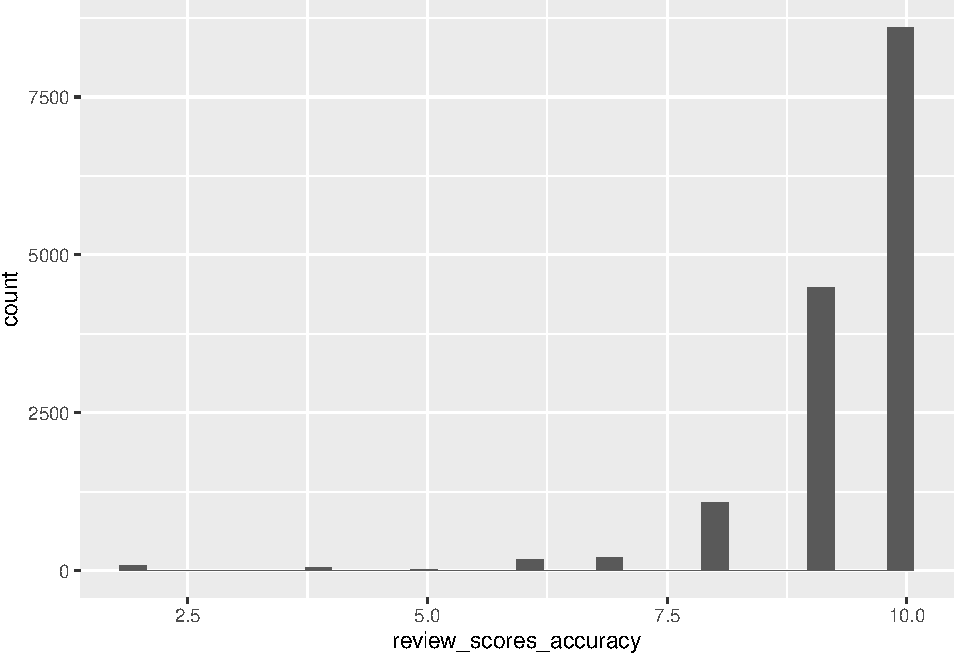
\includegraphics{anal_files/figure-latex/unnamed-chunk-9-44.pdf}

\begin{verbatim}
## Warning: Removed 5982 rows containing non-finite values (stat_boxplot).
\end{verbatim}

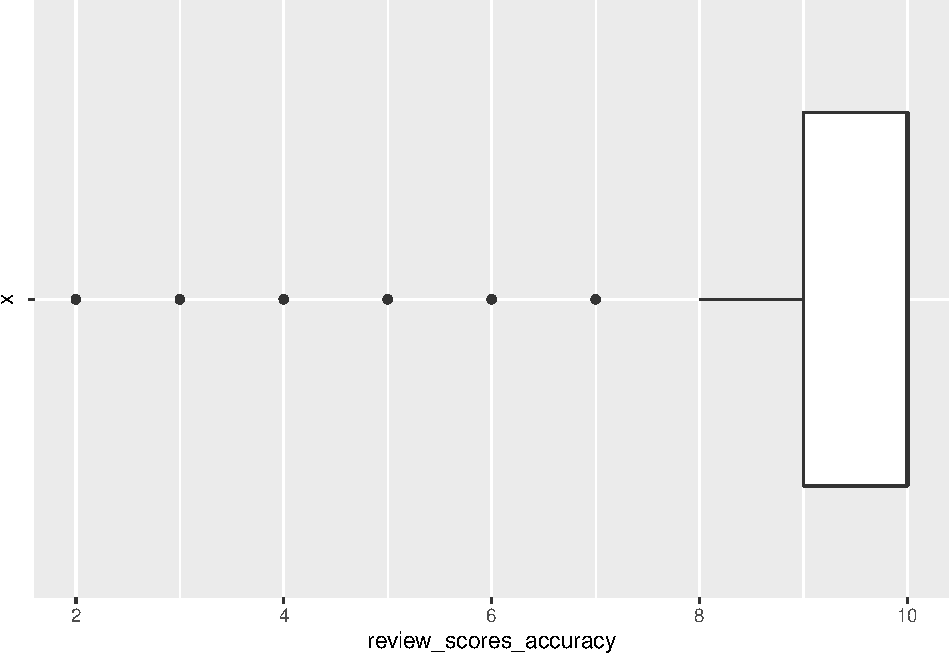
\includegraphics{anal_files/figure-latex/unnamed-chunk-9-45.pdf}

\begin{verbatim}
## [1] "Extended Summary Statistics"
##    Min. 1st Qu.  Median    Mean 3rd Qu.    Max.    NA's 
##   2.000   9.000  10.000   9.379  10.000  10.000    5982 
## [1] "sd:  1.04266849011004"
## [1] "vc:  0.111176384662649"
## [1] "variable  63 : review_scores_cleanliness"
\end{verbatim}

\begin{verbatim}
## `stat_bin()` using `bins = 30`. Pick better value with `binwidth`.
\end{verbatim}

\begin{verbatim}
## Warning: Removed 5980 rows containing non-finite values (stat_bin).
\end{verbatim}

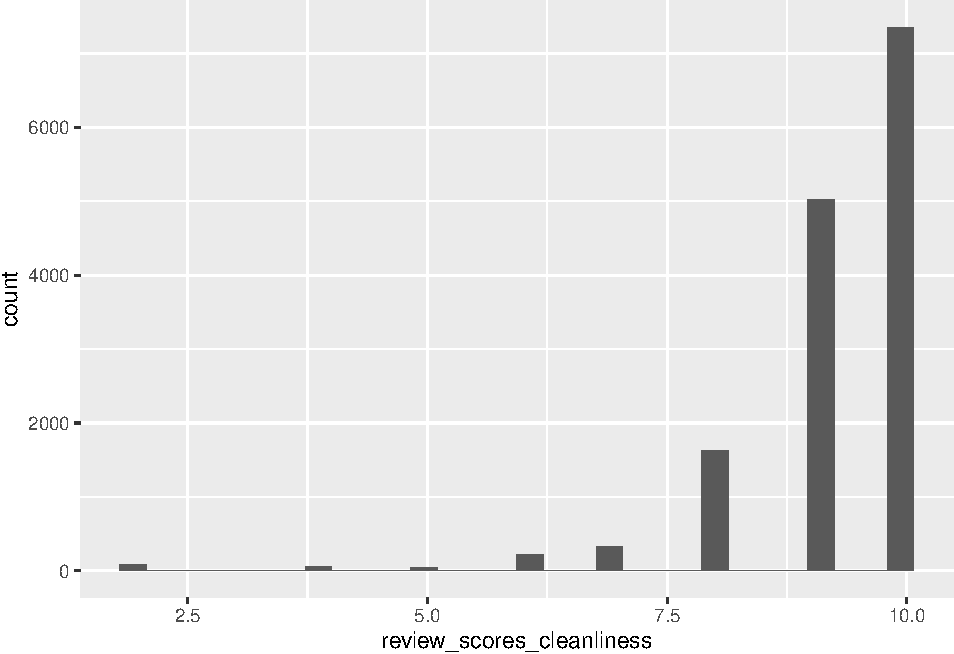
\includegraphics{anal_files/figure-latex/unnamed-chunk-9-46.pdf}

\begin{verbatim}
## Warning: Removed 5980 rows containing non-finite values (stat_boxplot).
\end{verbatim}

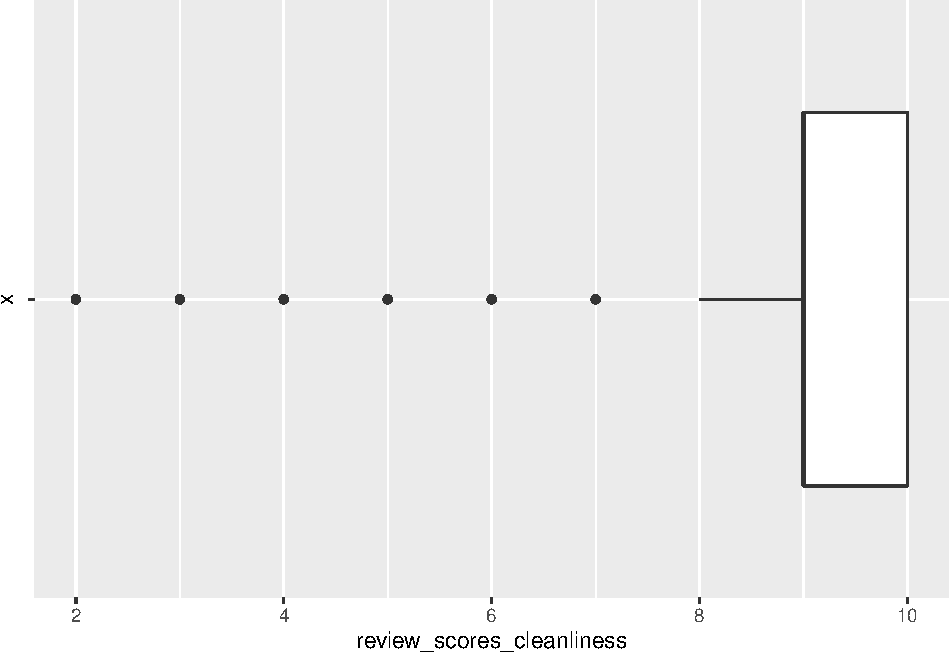
\includegraphics{anal_files/figure-latex/unnamed-chunk-9-47.pdf}

\begin{verbatim}
## [1] "Extended Summary Statistics"
##    Min. 1st Qu.  Median    Mean 3rd Qu.    Max.    NA's 
##   2.000   9.000   9.000   9.227  10.000  10.000    5980 
## [1] "sd:  1.10031287017275"
## [1] "vc:  0.119251994078246"
## [1] "variable  66 : review_scores_location"
\end{verbatim}

\begin{verbatim}
## `stat_bin()` using `bins = 30`. Pick better value with `binwidth`.
\end{verbatim}

\begin{verbatim}
## Warning: Removed 5985 rows containing non-finite values (stat_bin).
\end{verbatim}

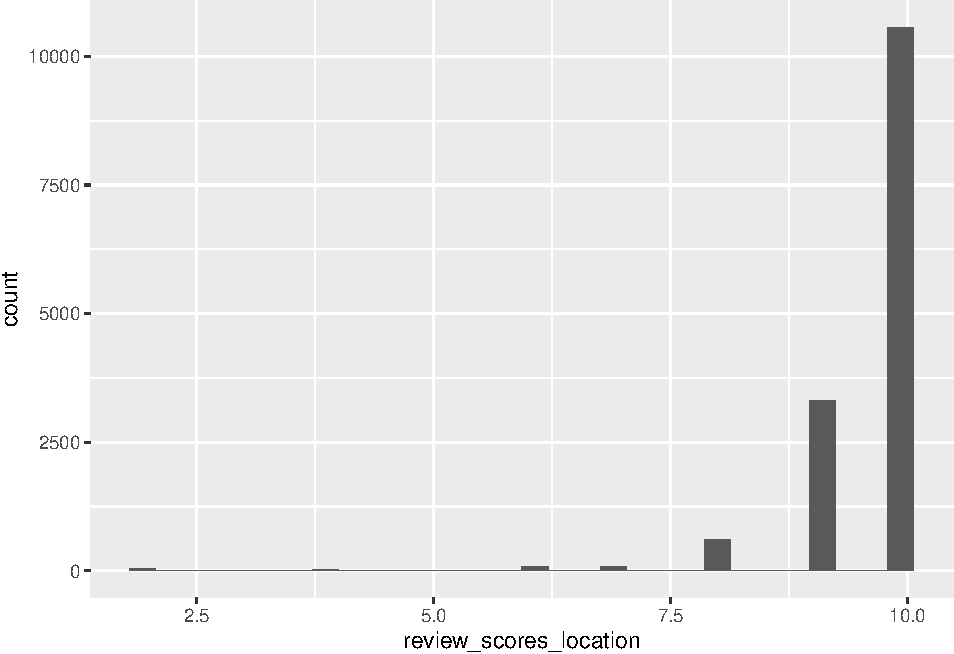
\includegraphics{anal_files/figure-latex/unnamed-chunk-9-48.pdf}

\begin{verbatim}
## Warning: Removed 5985 rows containing non-finite values (stat_boxplot).
\end{verbatim}

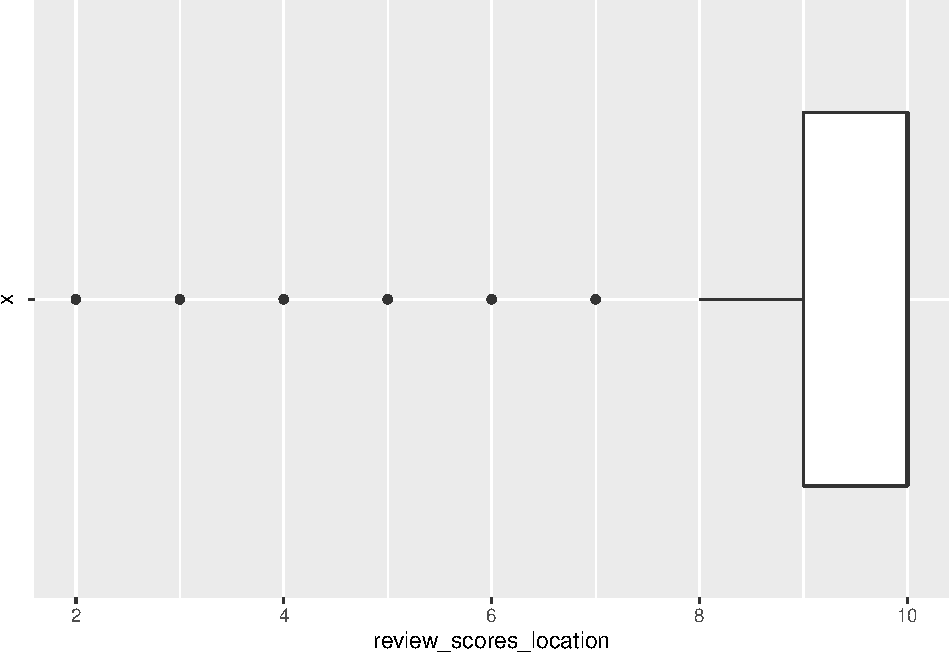
\includegraphics{anal_files/figure-latex/unnamed-chunk-9-49.pdf}

\begin{verbatim}
## [1] "Extended Summary Statistics"
##    Min. 1st Qu.  Median    Mean 3rd Qu.    Max.    NA's 
##   2.000   9.000  10.000   9.618  10.000  10.000    5985 
## [1] "sd:  0.788058627433689"
## [1] "vc:  0.0819339145567567"
## [1] "variable  67 : review_scores_value"
\end{verbatim}

\begin{verbatim}
## `stat_bin()` using `bins = 30`. Pick better value with `binwidth`.
\end{verbatim}

\begin{verbatim}
## Warning: Removed 5985 rows containing non-finite values (stat_bin).
\end{verbatim}

\includegraphics{anal_files/figure-latex/unnamed-chunk-9-50.pdf}

\begin{verbatim}
## Warning: Removed 5985 rows containing non-finite values (stat_boxplot).
\end{verbatim}

\includegraphics{anal_files/figure-latex/unnamed-chunk-9-51.pdf}

\begin{verbatim}
## [1] "Extended Summary Statistics"
##    Min. 1st Qu.  Median    Mean 3rd Qu.    Max.    NA's 
##   2.000   9.000   9.000   9.055  10.000  10.000    5985 
## [1] "sd:  1.0877510547065"
## [1] "vc:  0.120132968320041"
## [1] "variable  69 : instant_bookable"
\end{verbatim}

\includegraphics{anal_files/figure-latex/unnamed-chunk-9-52.pdf}
\includegraphics{anal_files/figure-latex/unnamed-chunk-9-53.pdf}

\begin{verbatim}
## [1] "Number of modalities:  2"
## [1] "Frequency table"
## 
## FALSE  TRUE 
##  9372 11331 
## [1] "Relative frequency table (proportions)"
## 
##    FALSE     TRUE 
## 0.452688 0.547312 
## [1] "Frequency table sorted"
## 
##  TRUE FALSE 
## 11331  9372 
## [1] "Relative frequency table (proportions) sorted"
## 
##     TRUE    FALSE 
## 0.547312 0.452688 
## [1] "variable  74 : reviews_per_month"
\end{verbatim}

\begin{verbatim}
## `stat_bin()` using `bins = 30`. Pick better value with `binwidth`.
\end{verbatim}

\begin{verbatim}
## Warning: Removed 5731 rows containing non-finite values (stat_bin).
\end{verbatim}

\includegraphics{anal_files/figure-latex/unnamed-chunk-9-54.pdf}

\begin{verbatim}
## Warning: Removed 5731 rows containing non-finite values (stat_boxplot).
\end{verbatim}

\includegraphics{anal_files/figure-latex/unnamed-chunk-9-55.pdf}

\begin{verbatim}
## [1] "Extended Summary Statistics"
##    Min. 1st Qu.  Median    Mean 3rd Qu.    Max.    NA's 
##   0.010   0.210   0.710   1.179   1.770  21.410    5731 
## [1] "sd:  1.28741924372801"
## [1] "vc:  1.09231185933215"
## [1] "variable  77 : host_since_season"
\end{verbatim}

\includegraphics{anal_files/figure-latex/unnamed-chunk-9-56.pdf}
\includegraphics{anal_files/figure-latex/unnamed-chunk-9-57.pdf}

\begin{verbatim}
## [1] "Number of modalities:  5"
## [1] "Frequency table"
## 
## Winter Spring Summer Autumn   <NA> 
##   4988   5411   5251   5031     22 
## [1] "Relative frequency table (proportions)"
## 
##      Winter      Spring      Summer      Autumn        <NA> 
## 0.240931266 0.261363087 0.253634739 0.243008260 0.001062648 
## [1] "Frequency table sorted"
## 
## Spring Summer Autumn Winter   <NA> 
##   5411   5251   5031   4988     22 
## [1] "Relative frequency table (proportions) sorted"
## 
##      Spring      Summer      Autumn      Winter        <NA> 
## 0.261363087 0.253634739 0.243008260 0.240931266 0.001062648 
## [1] "variable  75 : host_since_year"
\end{verbatim}

\includegraphics{anal_files/figure-latex/unnamed-chunk-9-58.pdf}
\includegraphics{anal_files/figure-latex/unnamed-chunk-9-59.pdf}

\begin{verbatim}
## [1] "Number of modalities:  14"
## [1] "Frequency table"
## 
## 2008 2009 2010 2011 2012 2013 2014 2015 2016 2017 2018 2019 2020 <NA> 
##    1   28  249 1179 1988 2395 1794 2392 2101 2126 2249 2973 1220    8 
## [1] "Relative frequency table (proportions)"
## 
##         2008         2009         2010         2011         2012         2013 
## 4.830218e-05 1.352461e-03 1.202724e-02 5.694827e-02 9.602473e-02 1.156837e-01 
##         2014         2015         2016         2017         2018         2019 
## 8.665411e-02 1.155388e-01 1.014829e-01 1.026904e-01 1.086316e-01 1.436024e-01 
##         2020         <NA> 
## 5.892866e-02 3.864174e-04 
## [1] "Frequency table sorted"
## 
## 2019 2013 2015 2018 2017 2016 2012 2014 2020 2011 2010 2009 <NA> 2008 
## 2973 2395 2392 2249 2126 2101 1988 1794 1220 1179  249   28    8    1 
## [1] "Relative frequency table (proportions) sorted"
## 
##         2019         2013         2015         2018         2017         2016 
## 1.436024e-01 1.156837e-01 1.155388e-01 1.086316e-01 1.026904e-01 1.014829e-01 
##         2012         2014         2020         2011         2010         2009 
## 9.602473e-02 8.665411e-02 5.892866e-02 5.694827e-02 1.202724e-02 1.352461e-03 
##         <NA>         2008 
## 3.864174e-04 4.830218e-05 
## [1] "variable  78 : host_response_rate_cat"
\end{verbatim}

\includegraphics{anal_files/figure-latex/unnamed-chunk-9-60.pdf}
\includegraphics{anal_files/figure-latex/unnamed-chunk-9-61.pdf}

\begin{verbatim}
## [1] "Number of modalities:  6"
## [1] "Frequency table"
## 
##  very low       low   average      high very high      <NA> 
##       588       240       487       996     11218      7174 
## [1] "Relative frequency table (proportions)"
## 
##   very low        low    average       high  very high       <NA> 
## 0.02840168 0.01159252 0.02352316 0.04810897 0.54185384 0.34651983 
## [1] "Frequency table sorted"
## 
## very high      <NA>      high  very low   average       low 
##     11218      7174       996       588       487       240 
## [1] "Relative frequency table (proportions) sorted"
## 
##  very high       <NA>       high   very low    average        low 
## 0.54185384 0.34651983 0.04810897 0.02840168 0.02352316 0.01159252 
## [1] "variable  79 : host_acceptance_rate_cat"
\end{verbatim}

\includegraphics{anal_files/figure-latex/unnamed-chunk-9-62.pdf}
\includegraphics{anal_files/figure-latex/unnamed-chunk-9-63.pdf}

\begin{verbatim}
## [1] "Number of modalities:  6"
## [1] "Frequency table"
## 
##  very low       low   average      high very high      <NA> 
##       852       379       713      1584     13737      3438 
## [1] "Relative frequency table (proportions)"
## 
##   very low        low    average       high  very high       <NA> 
## 0.04115346 0.01830653 0.03443945 0.07651065 0.66352703 0.16606289 
## [1] "Frequency table sorted"
## 
## very high      <NA>      high  very low   average       low 
##     13737      3438      1584       852       713       379 
## [1] "Relative frequency table (proportions) sorted"
## 
##  very high       <NA>       high   very low    average        low 
## 0.66352703 0.16606289 0.07651065 0.04115346 0.03443945 0.01830653
\end{verbatim}

}


% Enumerate which steps of the preprocessing process are used with your
% particular data (consider the steps proposed in slide 4 of Preprocessing
% Slides in Theme 2. Data Preparation. Remember that you have the whole
% complete information on preprocessing in the reference text from the
% linkSurvey of preprocessing. Reference paper (MIE 2001) from complementary
% materials section of Theme 2. Data Preparation)

% List and justify all decisions taken for each preprocessing step

% Additional descriptive statistics of variables that have been modified or
% created by preprocessing
\clearpage
\section{Preprocessing}
% vim: spell spelllang=en:
%! TEX root = **/main.tex

\subsection{Steps and Decisions}%
\label{sub:steps-decisions}

\subsubsection{Formatting issues, building software context}
We haven't encountered any formatting issues or problems with R
not recognising any rows, columns or variable types.

\subsubsection{Determining working matrix}
We discarded many variables from the original data set that didn't 
provide any useful information to our project such as URLs and ids or that couldn't be 
categorised or were uninteresting such as the host\_name, name 
and description of the listing, etc. Furthermore, some columns were duplicated with
different variable names, such as host\_listings\_count and 
host\_total\_listings\_count, we removed those redundancies as well.

\subsubsection{Identification and treatment of missing data}

\subsubsection{Identification and treatment of outliers}
When looking at the boxplots of most of the numerical variables in the dataset we can observe
that there are a few outliers. Some of them, although differing from the general 
distribution of the values are to be expected. For example the outliers we find in price,
beds or score could easily be explained (maybe they correlate to the room\_type variable)

On the other hand we also found some outliers that correspond to extreme values that are not
expected. For example in \texttt{maximum\_nights\_avg\_ntm} we found some rows with the value 2147483647,
which corresponds to the maximum int32 allowed. If we convert that value into years we would get a result 
that is unreasonable. 

We have decided to allow for some outliers as long as they are few and justifiable, in these cases we 
will try to correlate them to other variables. However in the cases when we encounter unreasonable 
values (3 rows) we have decided to treat these values as errors and discard the rows.

\subsubsection{Identification and treatment of errors}
\subsubsection{Feature selection/extraction, dimensional reduction}
\subsubsection{Instance selection}
\subsubsection{Data transformation}
\subsubsection{Derivation of new variables}
We derived some new variables from the data set in order to flourish new categorical variables.

First, starting with the host\_since variable, which gave us the date the host signed up to AirBnB
to list his property, we extracted two new variables: host\_since\_year and host\_since\_season,
both categorical. host\_since\_year categorizes the host sign up dates into their particular year and since . 
The variable host\_since\_season represents the season of the year during which
the host signed up. For the latter, the modalities are Winter, Spring, Summer and Autumn.

We have also categorized host\_response\_rate and host\_acceptance\_rate
as we converted them from a numerical variables measured in percentages to 
categorical ones with the following modalities: very low, low, average, 
high and very high. 

These were all the variable derivations we carried out in our data set for this 
project. They were all motivated by the necessity to have more categorical
variables in our data set, as it had plenty numerical and binary variables
but was short of categorical ones.

% Enumerate which steps of the preprocessing process are used with your
% particular data (consider the steps proposed in slide 4 of Preprocessing
% Slides in Theme 2. Data Preparation. Remember that you have the whole
% complete information on preprocessing in the reference text from the
% linkSurvey of preprocessing. Reference paper (MIE 2001) from complementary
% materials section of Theme 2. Data Preparation)

% List and justify all decisions taken for each preprocessing step

% Additional descriptive statistics of variables that have been modified or
% created by preprocessing


\end{document}
